\section{Owner Audit and Corrective Feedback}
\label{sec:exp-owner}

The preceding section measured what the pipeline believes; this one measures
what the room's occupant knows, and how that knowledge feeds back into the
graph. The room's occupant exhaustively labeled all 41 T3 clusters. Of the 31
verified-tier clusters, 6 were correct, 13 were real objects flattened to
\texttt{clutter}, 6 were structure-noise phantoms, 2 carried a wrong specific
label, and 3 were multi-object merges. The cause of the absorption is
identifiable: the room is a robotics testbed (mobile robots, manipulators,
charging stations, a disinfection robot), and none of these classes exist in
the classifier vocabulary. Three audit-driven mitigations follow (layers 4--5 of
Section~\ref{sec:corrective}). \emph{(i) Hybrid structure filter:} registering
every cluster against the exploration occupancy grid removes structure noise at
12/12 recall with 3 false positives (thin wall-flush real objects: a cabinet
leg, a poster stand); crucially, the wall-flush monitor bank survives, because
its 1.8~m height and per-segment depth separate it from the 3.2~m
floor-to-ceiling wall band that plane removal missed
(Figure~\ref{fig:structfilter}). \emph{(ii) Recovery re-verification:}
re-asking the verifier with \texttt{clutter} treated as unidentified plus a
candidate shortlist recovered 4 specific types at 4/5 precision; injecting
site vocabulary (robot classes) as candidates doubled recovery (9 correct) but
halved precision (8 wrong) through candidate anchoring---the TV became a
``conveyor belt'' when the shortlist ranked it first. \emph{(iii) Agreement
gating:} adopting a recovered label only when both passes agree, or when a
pass agrees with the cluster's own base label, yields five adoptions at 5/5
precision (two chairs, an office chair, a machine, and the TV) and resurrects
no owner-refuted phantom. Domain knowledge helps recall; only agreement makes
it safe. Refutations, corrections, and adopted labels were applied as a graph
revision through the same upsert mechanism as a re-scan: eight phantoms leave
the graph, five recovered types land, the TV becomes its region's key object,
the relation layer sheds nine noise-anchored edges, and re-deriving ring codes
heals the place layer end to end---the phantom-derived
\texttt{staircase\_landing} becomes \texttt{display\_briefing\_area}, the
keyboard-derived \texttt{workstation\_area} becomes \texttt{machine\_area},
and the seating region's recovered chairs turn
\texttt{cluttered\_seating\_area} into \texttt{seating\_area}. Owner feedback
thus propagates through all three layers of the model: object, relation, and
place.

\begin{figure}[!htb]
\centering
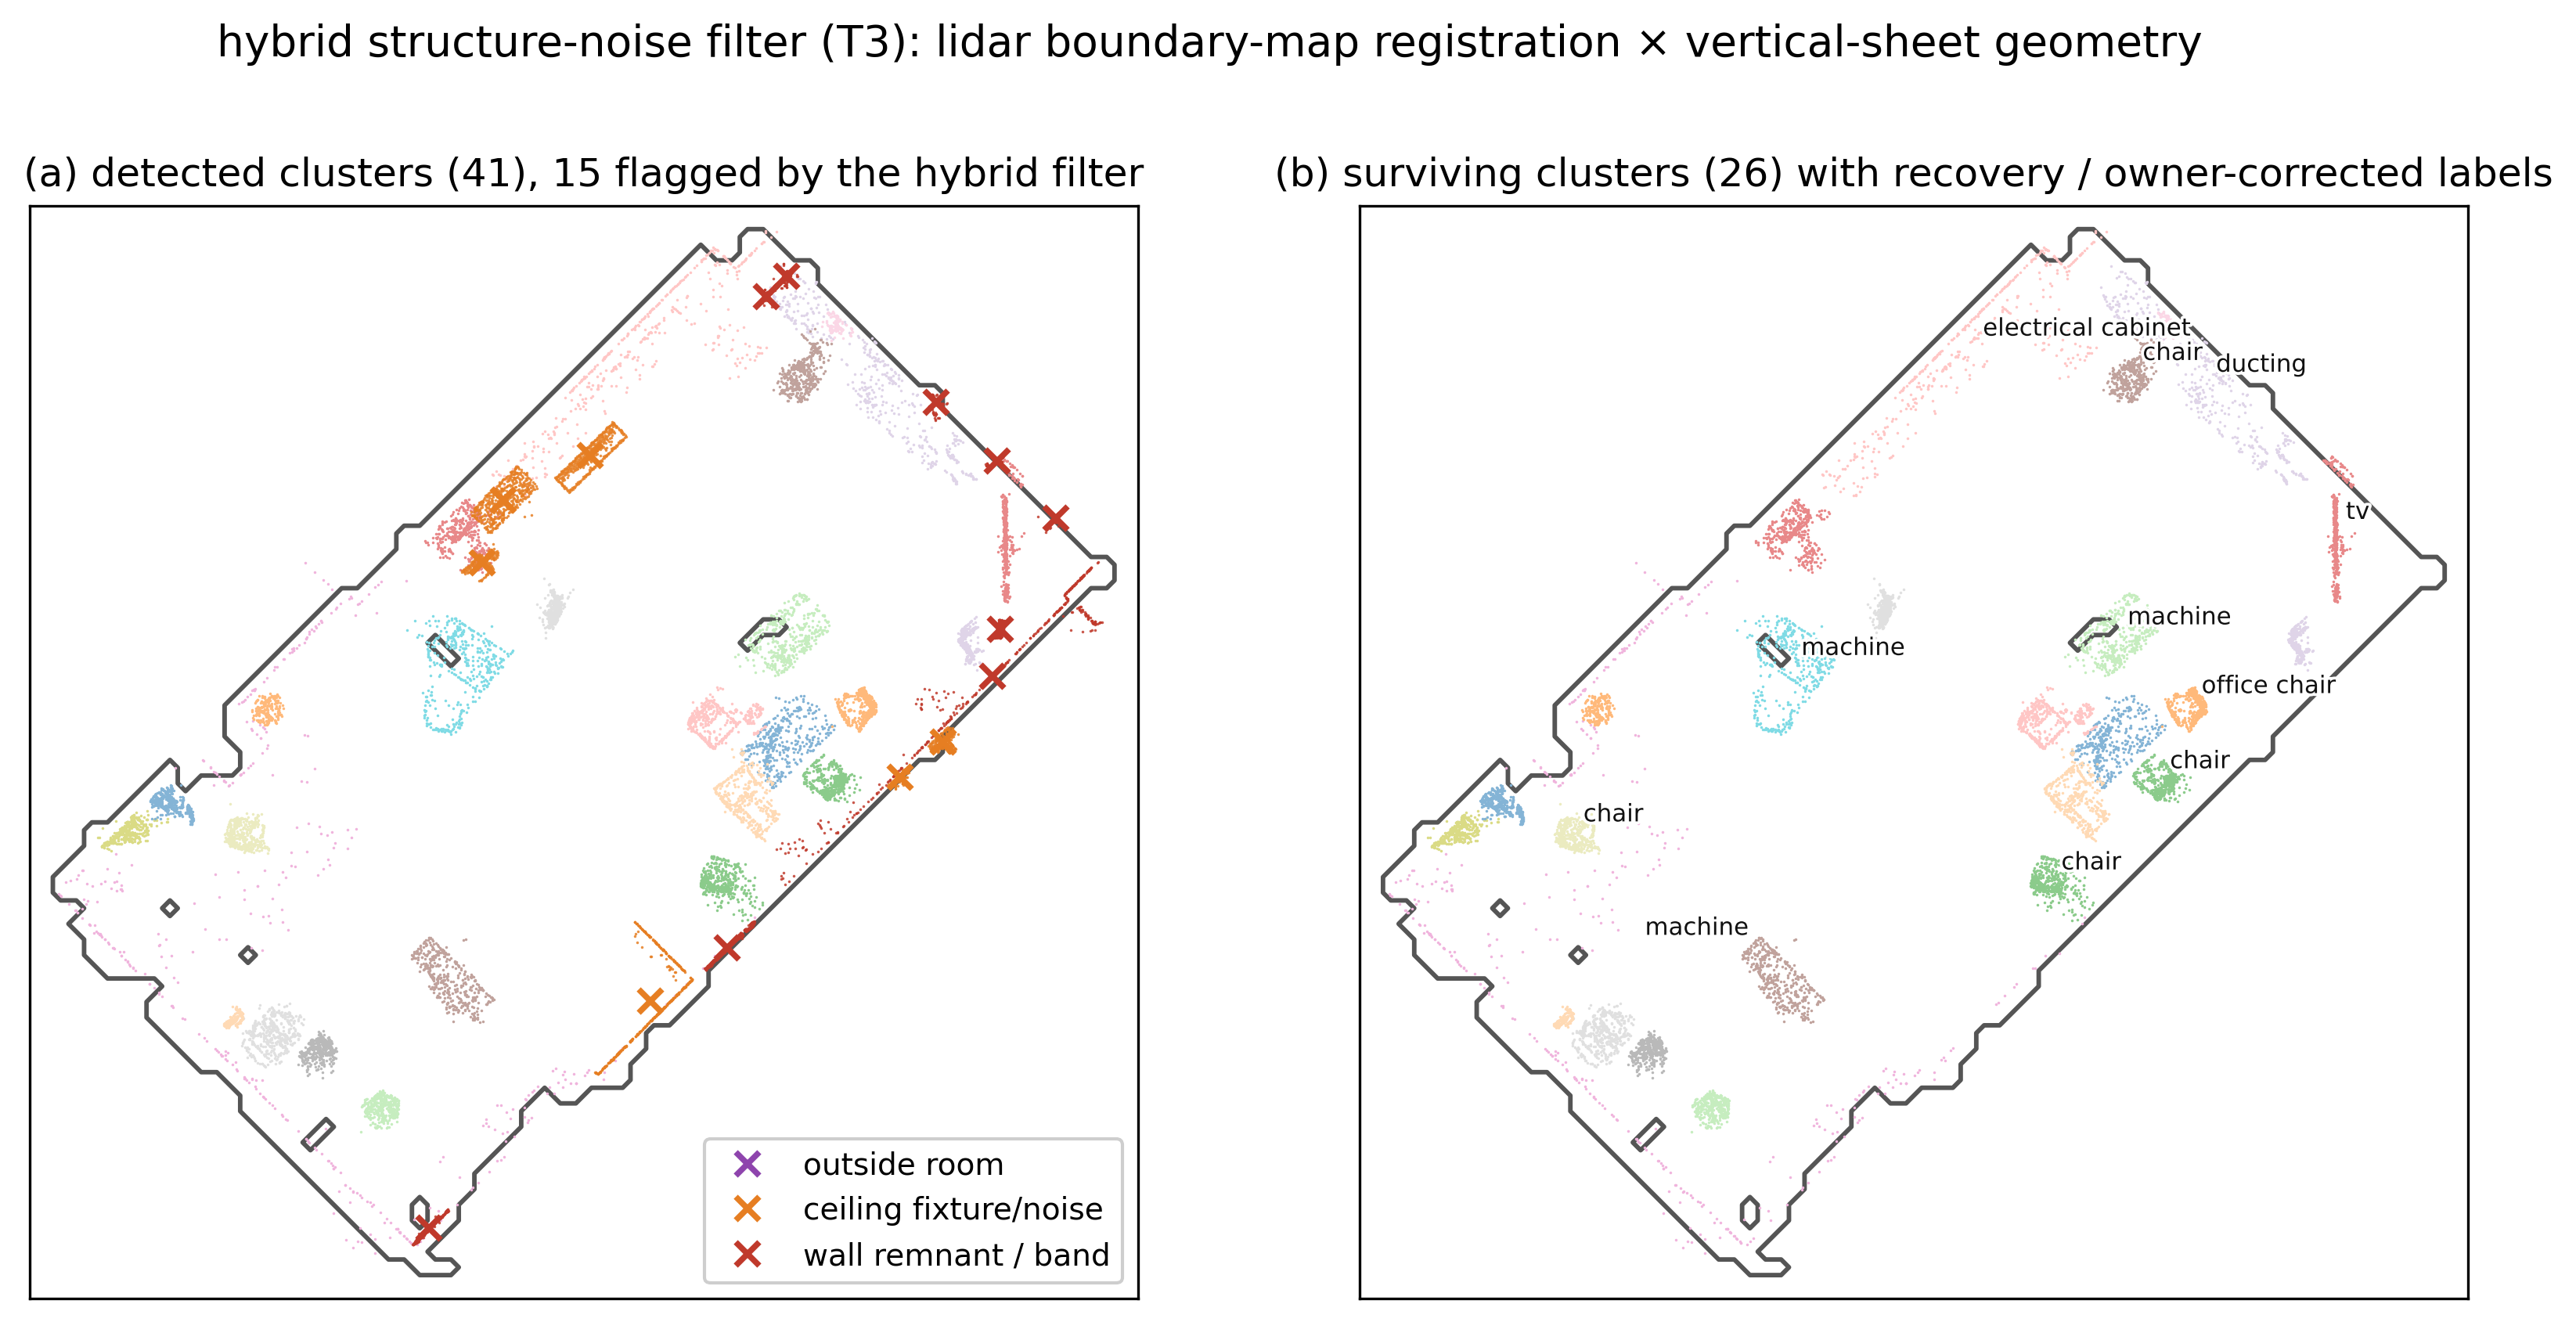
\includegraphics[width=\linewidth]{figures/ele_fig14_structure_filter.png}
\caption{Hybrid structure-noise filter on the T3 epoch. (a)~All 41 detected
clusters; the 15 flagged ones are colored by rule (wall remnant/band, ceiling
fixture/noise, outside the room boundary). (b)~The 26 survivors with recovery
and owner-corrected labels; the wall-flush monitor bank and wall-mounted
equipment survive.}
\label{fig:structfilter}
\end{figure}

Extending the audit loop through nine further revisions shows owner feedback
operating in all four directions the model supports. \emph{Restoration}: an
object the owner had refuted as absent was later declared present again (the
room changed between audits); a color-seeded carve at the owner-given corner
recovered a 319-point red cylinder that two-pass verification typed
\texttt{fire extinguisher}---the original failure was segmentation, not
classification, and owner ground truth is itself time-variant.
\emph{Refutation}: a raw-condition ensemble find was refuted as wall paint, the
halo around the hole left by the glossy black screen of the wall TV.
\emph{Label correction}: the correlated-bias tables and a poster stand were
corrected in place with the VLM verdict preserved in provenance.
\emph{Attribute correction}: wall-remnant clutter was marked immovable. The
live graph has accumulated thirteen revisions through the same mechanism, and
every transition, including the mistakes it corrects, is reconstructible from
node histories.

\section{Knowledge-Grounded Query Evaluation}
\label{sec:exp-query}

Four conditions are evaluated over identically constructed per-scene query
sets---48 items on the showroom, 32 on the robot hall (symbolic, explicit,
scene-level, and trap questions): (1)~\emph{LLM-only} (an unverified Stage-A
object dump, no verification), (2)~\emph{ungated KG}, (3)~\emph{verified-only
KG} (unverified nodes removed), and (4)~\emph{gated KG} (unverified retained
but structurally demoted). Each scene carries four trap questions about
objects that do not exist as labeled; on the showroom all four target
unverified-label phantoms, on the robot hall two target an unverified-label
phantom and two an \emph{escalation-verified} phantom, probing the gate's
verifier-quality bound. On the showroom (Table~\ref{tab:query},
Figure~\ref{fig:query}), grounding alone lifts accuracy from 52.1\% to 81.2\%
but blocks no traps; removing unverified content blocks all four traps at a
steep recall price (12 abstentions, 58.3\%); the gated condition is the balance
point---83.3\% with 3/4 traps blocked. The two leaks are mechanistically
distinct: on the showroom, one count-phrased trap slipped through the
quarantine itself, the model tallying a demoted node by reading its
\texttt{failedCandidateType} field; on the robot hall, the keyboard phantom is
escalation-verified, so it passes any status-based gate---gating is bounded by
verifier quality. The robot hall reproduces the ordering at lower absolute
levels because its end-to-end label errors propagate into every grounded
condition. At $n=48$/32 questions the gated-versus-ungated accuracy gap is a
single question on each scene, so the benchmark is diagnostic rather than
powered for significance; the case for gating rests on the mechanisms the
benchmark isolates---trap blocking, the abstention structure, and the direction
of the hallucination change---and on the mission-level consequences of
Section~\ref{sec:exp-missions}.

\begin{table}[htbp]
\centering
\caption{Query benchmark, four conditions. Acc.\ = accuracy, Hall.\ =
hallucination rate, Traps = trap questions blocked (of 4), Abst.\ =
abstentions. An abstention counts against accuracy but is not a hallucination.
Source: \emph{Electronics}~\cite{kim2026electronics}.}
\label{tab:query}
\small
\begin{tabular}{l c c c c c c c c}
\toprule
 & \multicolumn{4}{c}{\textbf{Showroom ($n=48$)}} & \multicolumn{4}{c}{\textbf{Robot hall ($n=32$)}} \\
\textbf{Condition} & Acc. & Hall. & Traps & Abst. & Acc. & Hall. & Traps & Abst. \\
\midrule
LLM-only & 52.1\% & 20.8\% & 2/4 & 13 & 50.0\% & 37.5\% & 4/4 & 4 \\
Ungated KG & 81.2\% & 18.8\% & 0/4 & 0 & 56.2\% & 43.8\% & 0/4 & 0 \\
Verified-only KG & 58.3\% & 16.7\% & 4/4 & 12 & 46.9\% & 40.6\% & 2/4 & 4 \\
Gated KG (proposed) & \textbf{83.3\%} & \textbf{16.7\%} & 3/4 & 0 & \textbf{59.4\%} & \textbf{40.6\%} & 2/4 & 0 \\
\bottomrule
\end{tabular}
\end{table}

\begin{figure}[!htb]
\centering
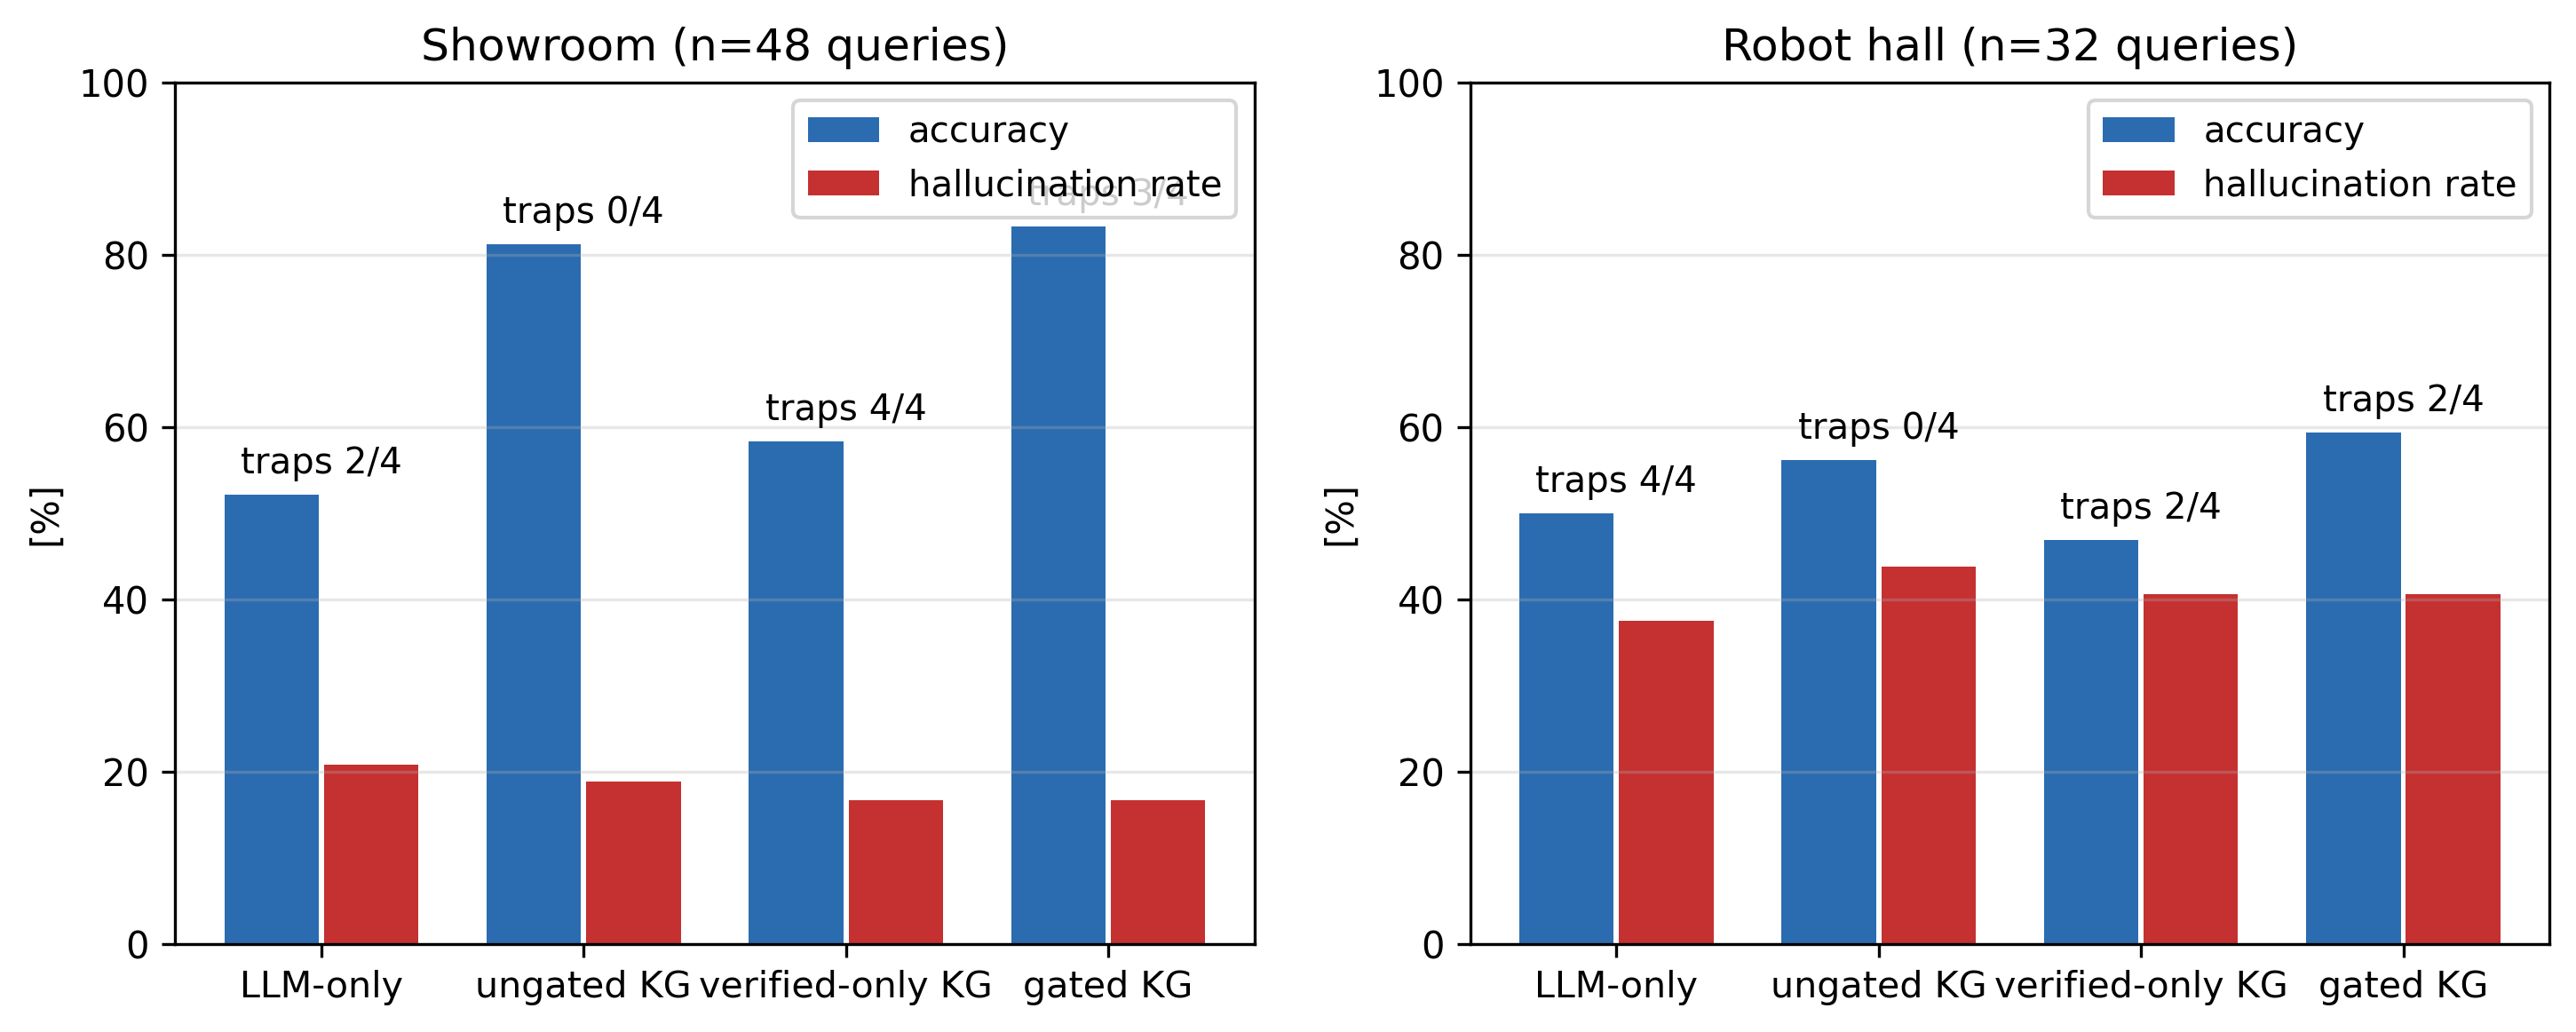
\includegraphics[width=0.9\linewidth]{figures/ele_fig7_query_benchmark.png}
\caption{Four-condition query benchmark with trap-question panel.}
\label{fig:query}
\end{figure}

\section{Incremental Update Evaluation}
\label{sec:exp-update}

\paragraph{Synthetic scenarios.}
Controlled edits of the room-scoped robot hall isolate matcher behavior
(Figure~\ref{fig:update}): (A)~unchanged repeat: 55/55 nodes carried, zero VLM
calls, zero identity switches; (B)~move: 1/1 moved with ID preserved;
(C)~remove+insert: exact absent/insert classification; (D)~occlusion: at 20\%
crop both affected objects still match, at 40\% matching fails into 2
false-absents + 2 false-news---the matcher's quantified breaking point. On the
combined-edit re-scan (move, insertion, and removal applied together),
selective re-verification re-ran Stage~B on only the two changed clusters: 26
of 822 VLM calls, \$0.23 versus \$7.37 for a full re-verification---3.1\% of
rebuild cost, and 0\% for scenario~A. The claim is scoped precisely: the 3.1\%
figure comes from a controlled same-quality re-scan where unchanged clusters
reproduce byte-identically; on the real T2$\rightarrow$T3 transition the scan
protocol itself changed, no cluster hash matched, and the epoch paid full
verification cost (\$3.54 for 41 clusters).

\begin{figure}[!htb]
\centering
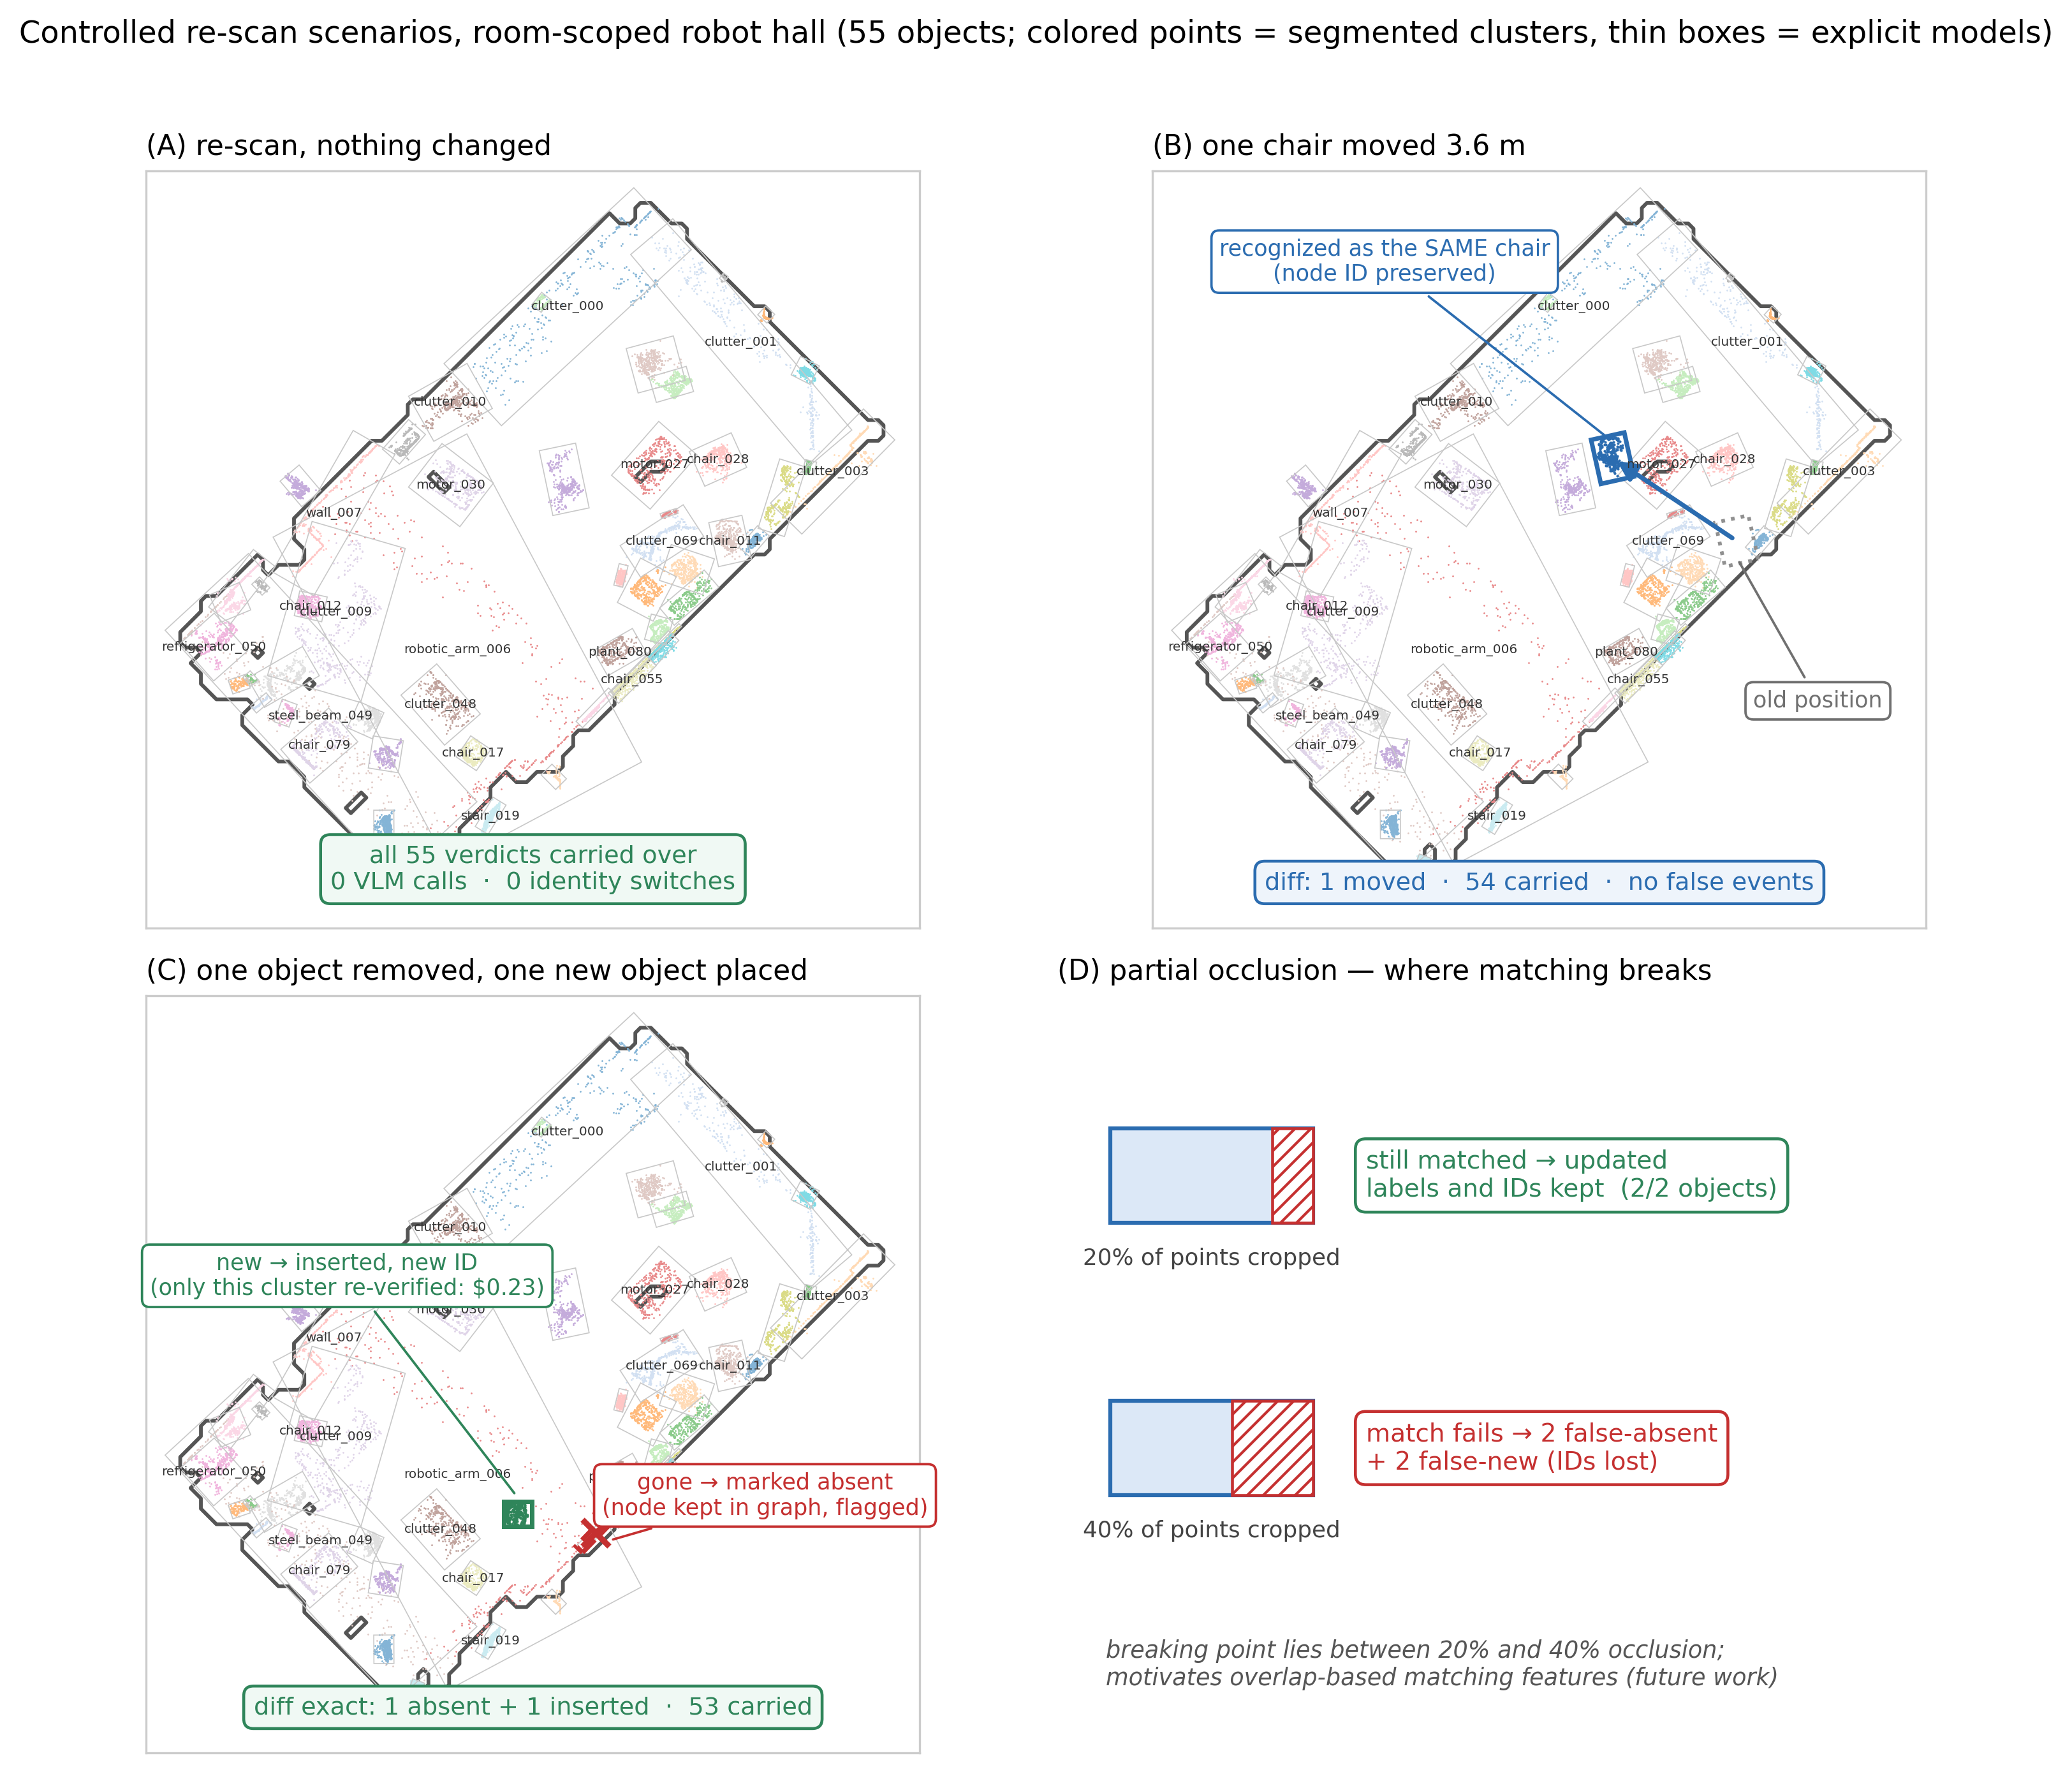
\includegraphics[width=0.9\linewidth]{figures/ele_fig8_incremental_update.png}
\caption{Controlled re-scan scenarios A--D (room-scoped robot hall, 55
objects), top-down view; each edited object is annotated with the matcher's
decision. (A)~A repeat scan carries all 55 verdicts at zero VLM cost. (B)~A
3.6~m chair move is classified \texttt{moved} with its node ID preserved.
(C)~A removed object is marked \texttt{absent} and a newly placed object is
\texttt{inserted}; only the insertion is re-verified. (D)~Partial occlusion:
both cropped objects still match at 20\%, but at 40\% matching fails.}
\label{fig:update}
\end{figure}

\paragraph{Real three-epoch study.}
The three epochs form a real update sequence: T1 (manual, June) $\rightarrow$
T2 (exploration, early July) $\rightarrow$ T3 (99.6\%-coverage exploration
with a controlled-change protocol, late July). Cross-epoch registration is
fully automatic (FPFH~\cite{rusu2009fpfh}+RANSAC then ICP~\cite{besl1992icp};
5.1~cm RMSE for T1$\rightarrow$T2, 4.2~cm for T3$\rightarrow$T2). The
T1$\rightarrow$T2 diff records the room's exhibition-to-test-hall
reorganization (updated 4 / moved 3 / inserted 48 / absent 31; among the moves,
a fire extinguisher displaced 3.0~m) and motivated the generic-type exclusion
in the move pass. The T2$\rightarrow$T3 diff (matched 9 / moved 1 / inserted 31
/ absent 45, Figure~\ref{fig:epochs}) sits on top of measured natural drift:
only 65\% of in-room object geometry is mutually supported at 10~cm between the
two scans, taken two weeks apart. To score the real transitions without circular
reference to the matcher, an independent correspondence reference was built by
bidirectional point overlap between epochs (4 strong and 6 partial static
pairs for T1$\rightarrow$T2, 7 strong and 5 partial for T2$\rightarrow$T3).
Matching accuracy on strong pairs is 2/4 and 4/7; \textbf{identity switches
are zero on both transitions}---every miss is a fragmentation error in which
re-segmentation changed an extent beyond the 30\% tolerance, so the object was
marked absent and re-inserted under a new ID, never associated with the wrong
object. Strict false-new and false-absent counts are 2/2 and 3/3, and all
three recorded \texttt{moved} claims are consistent with the reference (the
chair move is additionally owner-confirmed). Against the controlled-change
protocol, the system detected 2/2 physical changes at geometry level: the
moved chair is the epoch's only \texttt{moved} node (0.64~m, ID preserved
since T1), and the introduced floor fan was correctly \texttt{inserted} but
typed \texttt{clutter}. The fire extinguisher, pump, industrial robot, and
several chairs retain their minted IDs through both reorganizations, and the
place layer re-derives per-epoch names on the same regions (exhibition-era
\texttt{machine\_access\_area} $\rightarrow$ test-era
\texttt{machine\_operator\_station}) at about \$0.03 per epoch.

\begin{figure}[!htb]
\centering
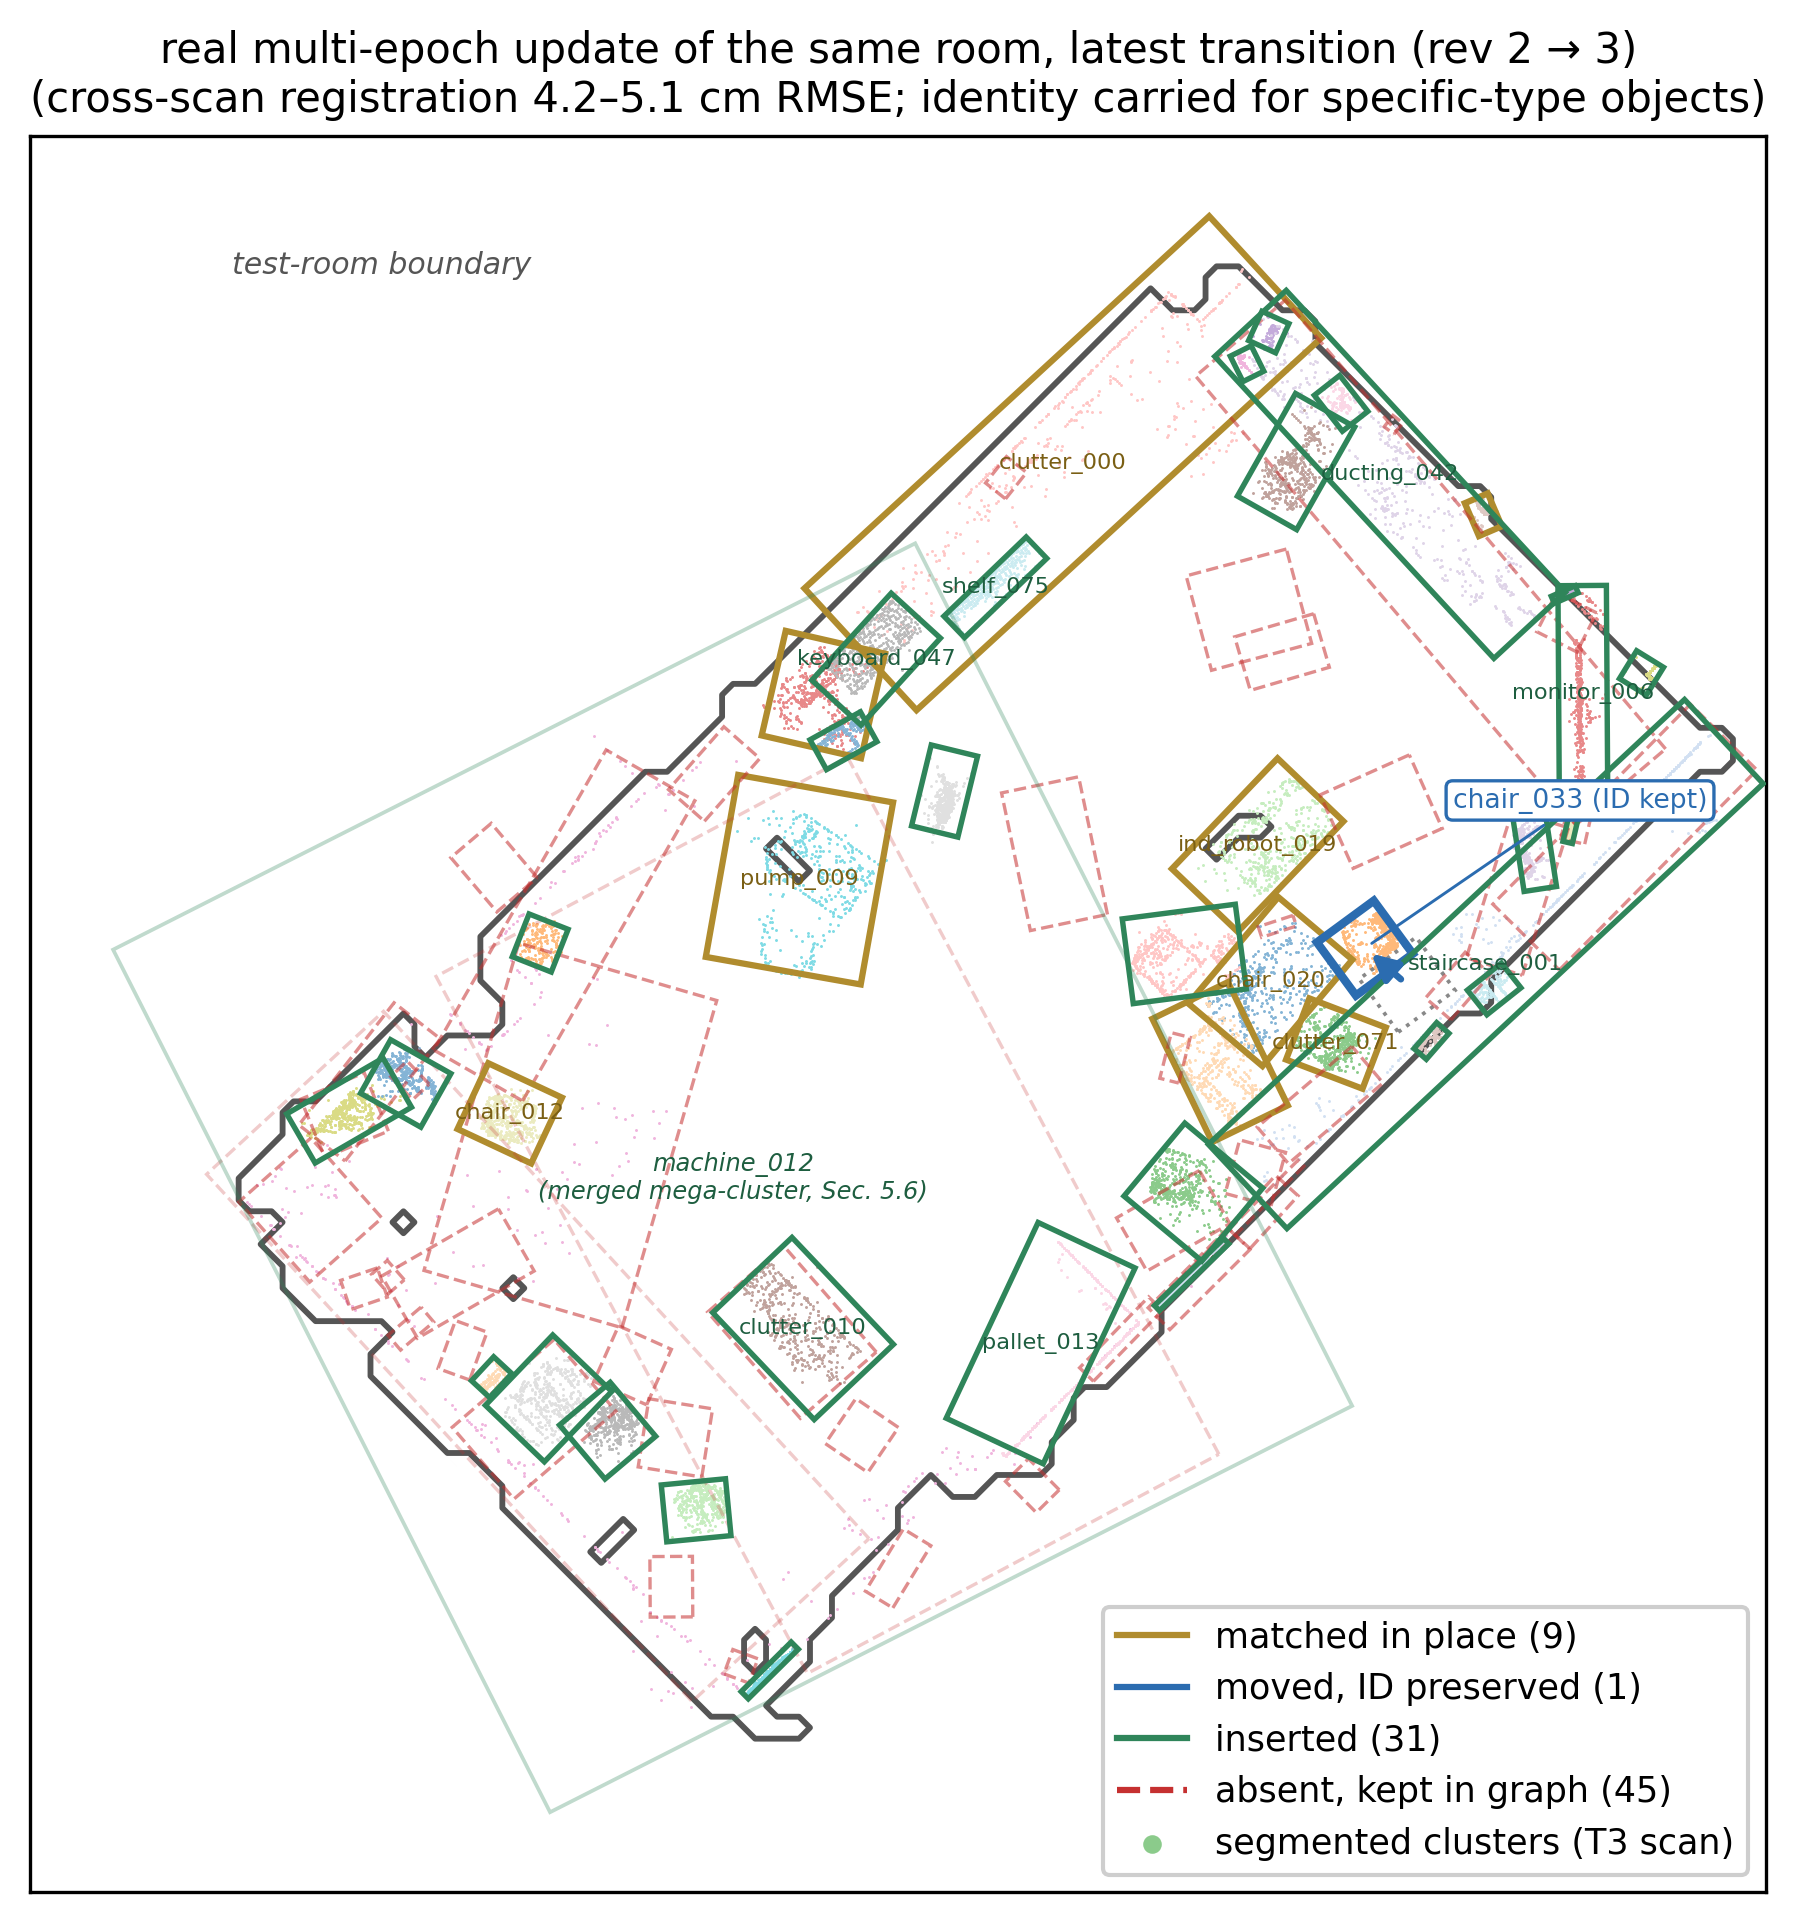
\includegraphics[width=0.9\linewidth]{figures/ele_fig9_two_epoch_update.png}
\caption{Real multi-epoch update, latest transition (T2$\rightarrow$T3),
top-down view: yaw-rotated node footprints colored by diff state (matched,
moved with ID preserved, inserted, absent). Oversized footprints of merged
mega-clusters are faded.}
\label{fig:epochs}
\end{figure}

\section{Retrospective End-to-End Replay}
\label{sec:exp-endtoend}

After the corrective machinery stabilized, the entire pipeline was re-run from
the raw T3 scan with no owner input at execution time and scored against the
live knowledge graph---by then a 46-object inventory embodying every owner
restoration, refutation, and correction. Because the corrective mechanisms were
developed from failures observed in this same environment, this is a
retrospective replay on the development scene, not an independent
generalization test: an independent \emph{run} on a non-independent
\emph{scene}. The cafeteria is the only scene independent in both senses, and
one corrective layer transfers mechanically to it: applying the hybrid
structure filter to the cafeteria with its T3 rules frozen flags both
ceiling-noise clusters with zero false positives, while the seven carpet
floor-noise clusters fall outside its rule families entirely.
Table~\ref{tab:layers} reports cumulative geometric recall as each automated
layer is enabled. The verified path alone recovers 28\%; diffuseness-gated
re-splitting nearly doubles it; the wall-compound gate (which self-triggers on
the monitor wall) and the structure-condition ensemble bring automated recall
to 85\%. Type accuracy saturates far lower ($\sim$31\% of recalled
objects)---the label bottleneck is the correlated verifier bias, and closing
it is precisely the owner layer's role. For calibration within the lineage's
own reporting style, DK-SMF reports 78--81\% detection accuracy against
predefined ground-truth objects in its RGB-D environments~\cite{joo2025dksmf};
the 85\% here is measured against an owner-audited inventory that includes
partially scanned and wall-flush objects, though the sensing modality and
ground-truth protocols differ. Each added layer admits more candidate
clusters, so automated recall is bought with review burden---exactly the
owner-review efficiency the model should optimize.

\begin{table}[htbp]
\centering
\caption{Cumulative automated recall of the full re-run against the
owner-corrected 46-object graph (no owner input in the run itself).}
\label{tab:layers}
\begin{tabular}{l c c}
\toprule
\textbf{Automated layers (cumulative)} & \textbf{GT recall} & \textbf{In-room precision} \\
\midrule
Verified path (backbone + verification) & 13/46 (28\%) & 37\% \\
+ diffuseness re-split & 26/46 (57\%) & 53\% \\
+ wall-compound gate & 36/46 (78\%) & 60\% \\
+ structure-condition ensemble & 37/46 (80\%) & 49\% \\
+ wall-compound panel square-up & \textbf{39/46 (85\%)} & 51\% \\
\bottomrule
\end{tabular}
\end{table}

\section{Ablation, Verifier Comparison, and Cross-Floor Stress Scene}
\label{sec:exp-ablation}

\paragraph{Gating style, pose context, and vocabulary.}
Instructing the model to respect verification status blocks 1/4 traps;
structural demotion blocks 4/4 under identical prompts in this isolated
comparison (versus 3/4 end to end)---the single strongest argument that
reliability must live in the data contract, not in instructions. Injecting
mounting-height context removed all three phantom ceiling keyboards in its
pilot, but applying it to every object \emph{reduced} escalated accuracy
($88.9\%\rightarrow75.0\%$), so it is deployed only as a targeted defense
and, later, as the coarse height-level attribute. Swapping the
Stage-A classifier vocabulary ranks generic-30 (66.7\%) above curated-20
(48.7\%) and above the owner-derived 18-term set (33.3\%): narrowing the prompt
set toward the deployment vocabulary \emph{hurts} the embedding-level
classifier, confirming the domain gap that motivates VLM verification.
Removing the provisional label from the verifier's context collapses
decisiveness (trigger rate $58\%\rightarrow90\%$, unanimity
$21\rightarrow5$ objects) and lowers escalated accuracy to 38.9\%: Stage~B is a
verifier of hypotheses, and the provisional label is load-bearing context,
which is why label adoption is agreement-gated and owner-auditable rather than
trusted outright.

\paragraph{Verifier model.}
Running the identical Stage-B protocol across five commercial verifiers (two
vendors, three tiers, two generations) makes escalation an economic instrument
(Table~\ref{tab:vlmcmp}): call volume tracks verifier decisiveness
monotonically (247 to 383 calls as unanimous verifications fall from 26 to 9).
Within a generation, the smaller tier splits more votes and resolves fewer,
inflating call volume by 14\% and eroding part of its nominal per-token
price advantage; all three current-generation frontier models tie on type
accuracy against the owner inventory (7/13) but differ twofold in the escalations
they need (9 versus 18); and the ranking is generation-dominated, not vendor-dominated.
Escalation volume is thus a label-free, online proxy for verifier decisiveness
on the deployment's own data---a practical criterion for verifier selection
under cost constraints---but not a proxy for accuracy: re-running both main
scenes under the most decisive model lowers escalation triggers (58\%
$\rightarrow$ 50\%, 51\% $\rightarrow$ 33\%) but also unanimous precision
(100\% $\rightarrow$ 91.7\%, 94.4\% $\rightarrow$ 83.3\%), re-distributing error
mass from indecision into confident under-labeling. Verifier upgrades change
\emph{where} errors live rather than uniformly removing them, which is why the
framework treats verification as tiered evidence behind a gate: the tier
structure, the escalation economics, and the owner loop survive a verifier
swap; the specific precision figures do not.

\begin{table}[htbp]
\centering
\caption{Verifier-model comparison: identical Stage-B late fusion +
escalation on the same 35 in-room T3 clusters, scored against the
owner-corrected graph. Type-correct = canonical-synonym match on the clusters
that geometrically match a ground-truth object; cost at vendor list rates of
August 2026.}
\label{tab:vlmcmp}
\footnotesize\setstretch{1.15}
\begin{tabular}{l c c c c c c}
\toprule
\textbf{Verifier} & Verified & Esc.-resolved & Unverified & Type-correct & Calls & Cost \\
\midrule
Claude Sonnet 5 & \textbf{26} & 3 & \textbf{6} & \textbf{7/13} & \textbf{247} & \$2.49 \\
GPT-5.6 & 21 & 7 & 7 & \textbf{7/13} & 287 & \$0.11 \\
Claude Opus 5 & 17 & 8 & 10 & \textbf{7/13} & 319 & \$5.28 \\
Claude Sonnet 4.6 & 15 & 6 & 14 & 6/13 & 335 & \$3.00 \\
Claude Haiku 4.5 & 9 & 9 & 17 & 5/13 & 383 & \$1.13 \\
\bottomrule
\end{tabular}
\end{table}

\paragraph{Cross-floor stress scene.}
The cafeteria scene probes the same protocol on a furnishing domain the
campaign never saw: carpeted floor, fabric sofa booths, planter partitions
(Figure~\ref{fig:cafe}). The backbone transfers mechanically---57~M points to
28 clusters in 13.5~s after an automatic wall-normal yaw alignment---but
verification does not (Table~\ref{tab:cafe}): escalated accuracy reaches only
35\% against confirmed owner ground truth, and unanimous precision falls to
57.1\%, with two unanimous keyboard phantoms on carpet-noise clusters. The
errors are structured: the scene's dominant object family---the sofas---enters
the pipeline pre-broken, split into five cushion fragments and two sofa--table
merges, and every one is absorbed; carpet pile leaves seven residual
floor-noise clusters above the RANSAC floor plane, the floor-material analogue
of the ceiling remnants; and the confidence gate quarantines 9 of the 16 wrong
labels as unverified while the unanimous errors pass. Two upgrades applied
factorially act on different error classes: re-rendering the identical view
sets from full-resolution points repairs \emph{whole-object} ambiguity (the
keyboard phantoms vanish, both chairs and both doors recover), and the
verifier upgrade adds accuracy on top of whichever source it is given
($35\rightarrow45\%$ on voxel, $40\rightarrow60\%$ on full-resolution sets).
Symmetric controls that re-render both industrial scenes from full-resolution
points \emph{reverse} the effect (showroom escalated accuracy
$88.9\rightarrow80.6\%$; robot hall $84.4\rightarrow68.8\%$), because added
texture invites over-specific labels; the main campaign's voxel-source
protocol therefore stands as the right default for the industrial scenes.
What neither lever reaches is fragmentation: the seven sofa clusters are
absorbed in all four cells. Segmentation bounds what any verifier can see;
render quality bounds what a given verifier resolves; the model generation
buys accuracy only on top of both. Tier precision is therefore a scene- and
domain-scoped measurement, to be re-estimated per deployment via a small
owner-confirmed probe set, rather than a property of the architecture.

\begin{table}[htbp]
\centering
\caption{Cafeteria stress scene: verification under verifier $\times$ render
source (identical 512-px multi-view protocol). Accuracy is escalated accuracy
on confirmed GT ($n=20$; the fragment-excluded column drops the five confirmed
sofa-fragment clusters, $n=15$). In every cell, 0 of the 7 sofa clusters are
recovered.}
\label{tab:cafe}
\begin{tabular}{l l c c c c}
\toprule
\textbf{Verifier} & \textbf{Render source} & Esc.\ acc. & (excl.\ fragments) & Unan.\ prec. & Trigger \\
\midrule
Sonnet 4.6 & 3~cm voxel cloud & 35.0\% & 46.7\% & 57.1\% & 68\% \\
Sonnet 4.6 & full-resolution & 40.0\% & 53.3\% & 62.5\% & 60\% \\
Sonnet 5 & 3~cm voxel cloud & 45.0\% & 60.0\% & 66.7\% & 40\% \\
Sonnet 5 & full-resolution & \textbf{60.0\%} & \textbf{80.0\%} & \textbf{80.0\%} & 52\% \\
\bottomrule
\end{tabular}
\end{table}

\begin{figure}[!htb]
\centering
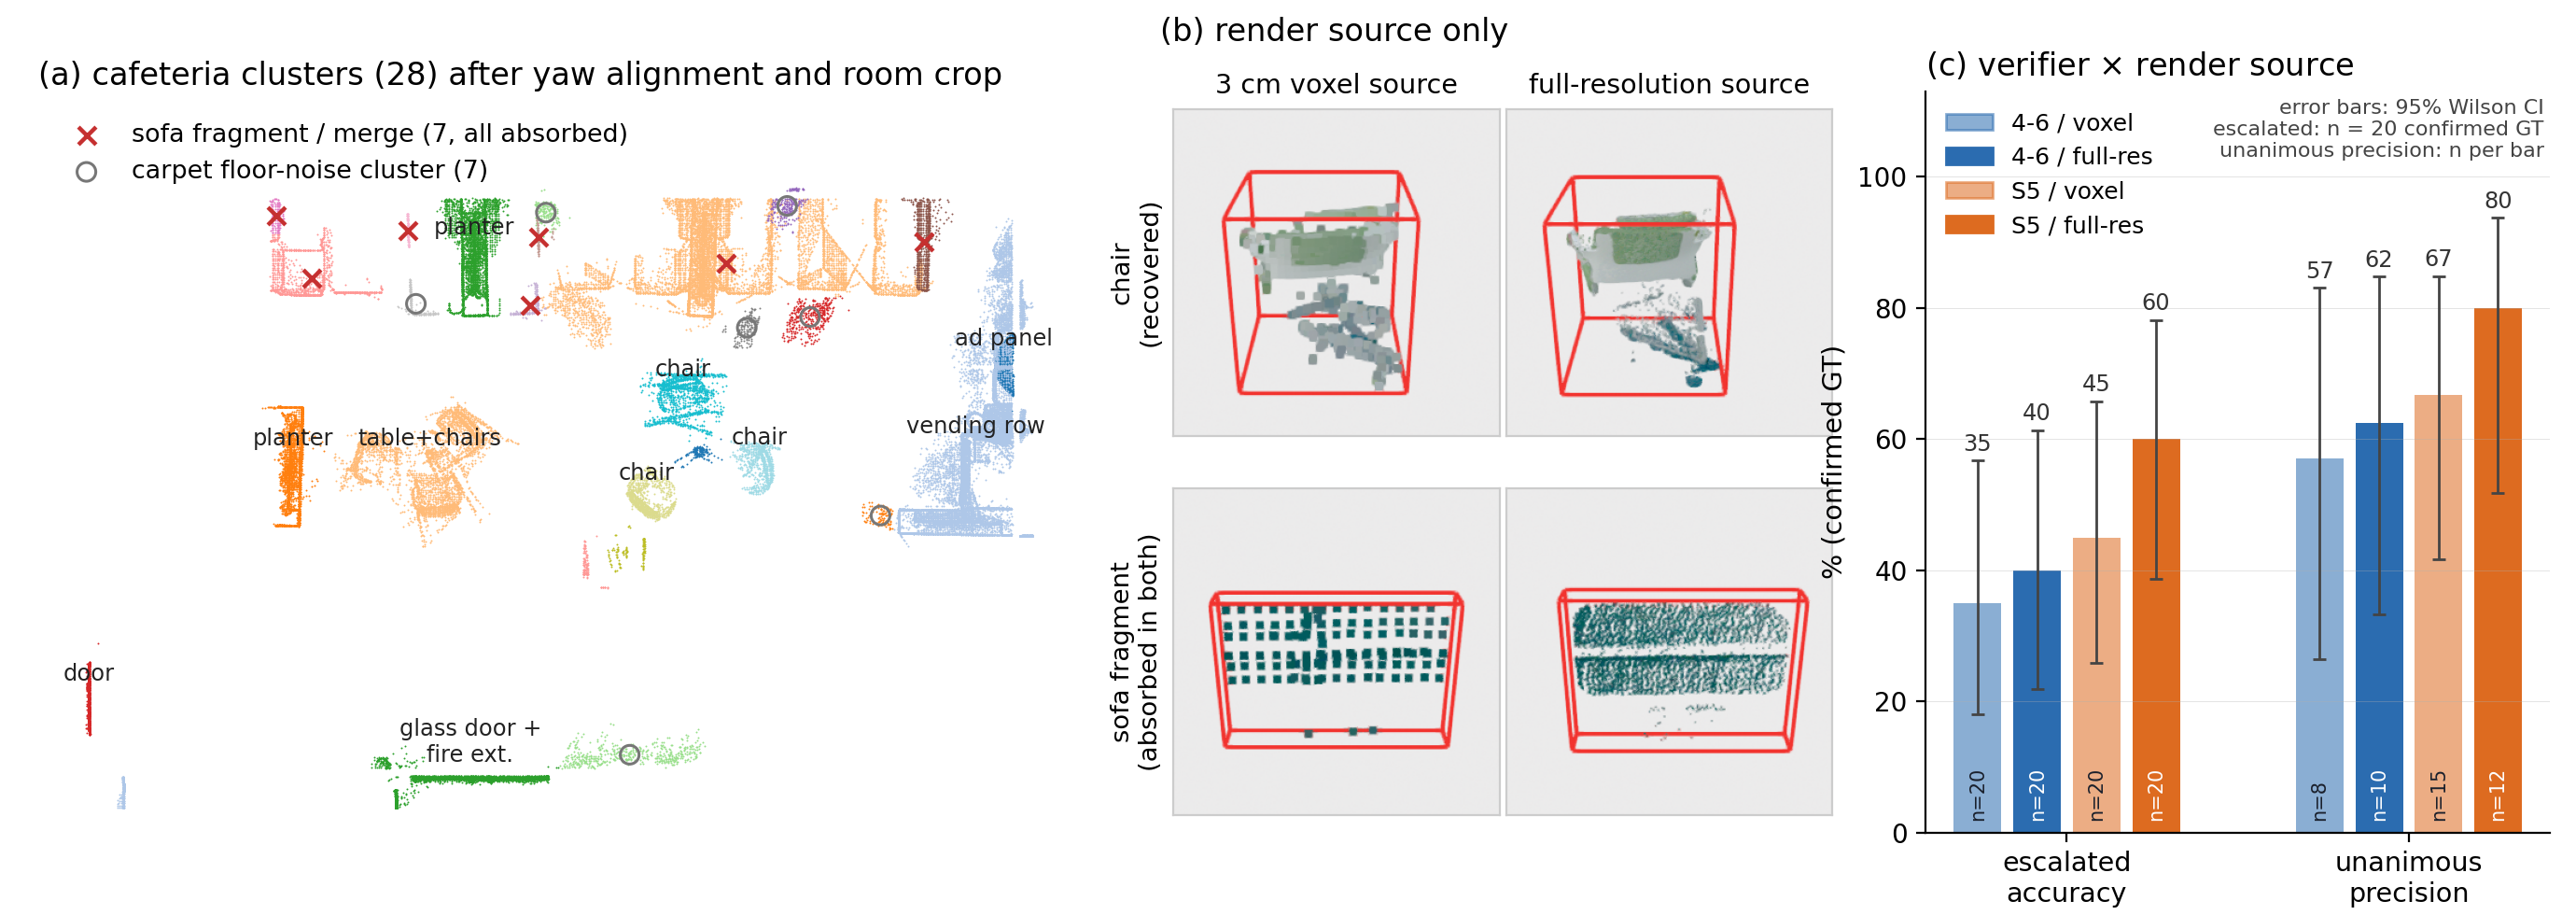
\includegraphics[width=\linewidth]{figures/ele_fig17_cafe_stress.png}
\caption{Cafeteria stress scene. (a)~The 28 clusters after automatic yaw
alignment and room crop; crosses mark the seven sofa fragments/merges,
circles the seven carpet floor-noise clusters. (b)~One cluster rendered from
the 3~cm working cloud (left) and from full-resolution re-associated points
(right): the chair (top) is recovered by the render-source change alone; the
sofa fragment (bottom) is not. (c)~Escalated accuracy and unanimous precision
across verifier $\times$ render source; error bars are 95\% Wilson intervals.}
\label{fig:cafe}
\end{figure}

\paragraph{Cost and latency.}
VLM verification is the only paid stage: full verification averages
$\sim$\$0.09 per object (\$3.63 for a 38-cluster run and \$7.37 for the
86-cluster robot-hall detection set, all calls included), and the incremental
design changes the cost model qualitatively (an identical-input repeat scan
costs \$0). Wall-clock time is equally bounded on the workstation: the full
deterministic backbone---loading the 68.6~M-point E57, 3~cm downsampling,
ten-plane removal, decomposition, and remnant filtering---completes in 29~s
(8.1~GB peak memory), rendering the four-view sets takes 99~s for 88 objects,
and verification with escalation runs in 7.7~min for a 50-object scene at six
concurrent calls, so the complete semantic modeling of a scene finishes in
well under ten minutes end to end. Verification is offline; no VLM call sits
on a robot's control path. Figure~\ref{fig:semmap} visualizes the resulting
semantic map with the confidence gate visible in the map itself.

\begin{figure}[!htb]
\centering
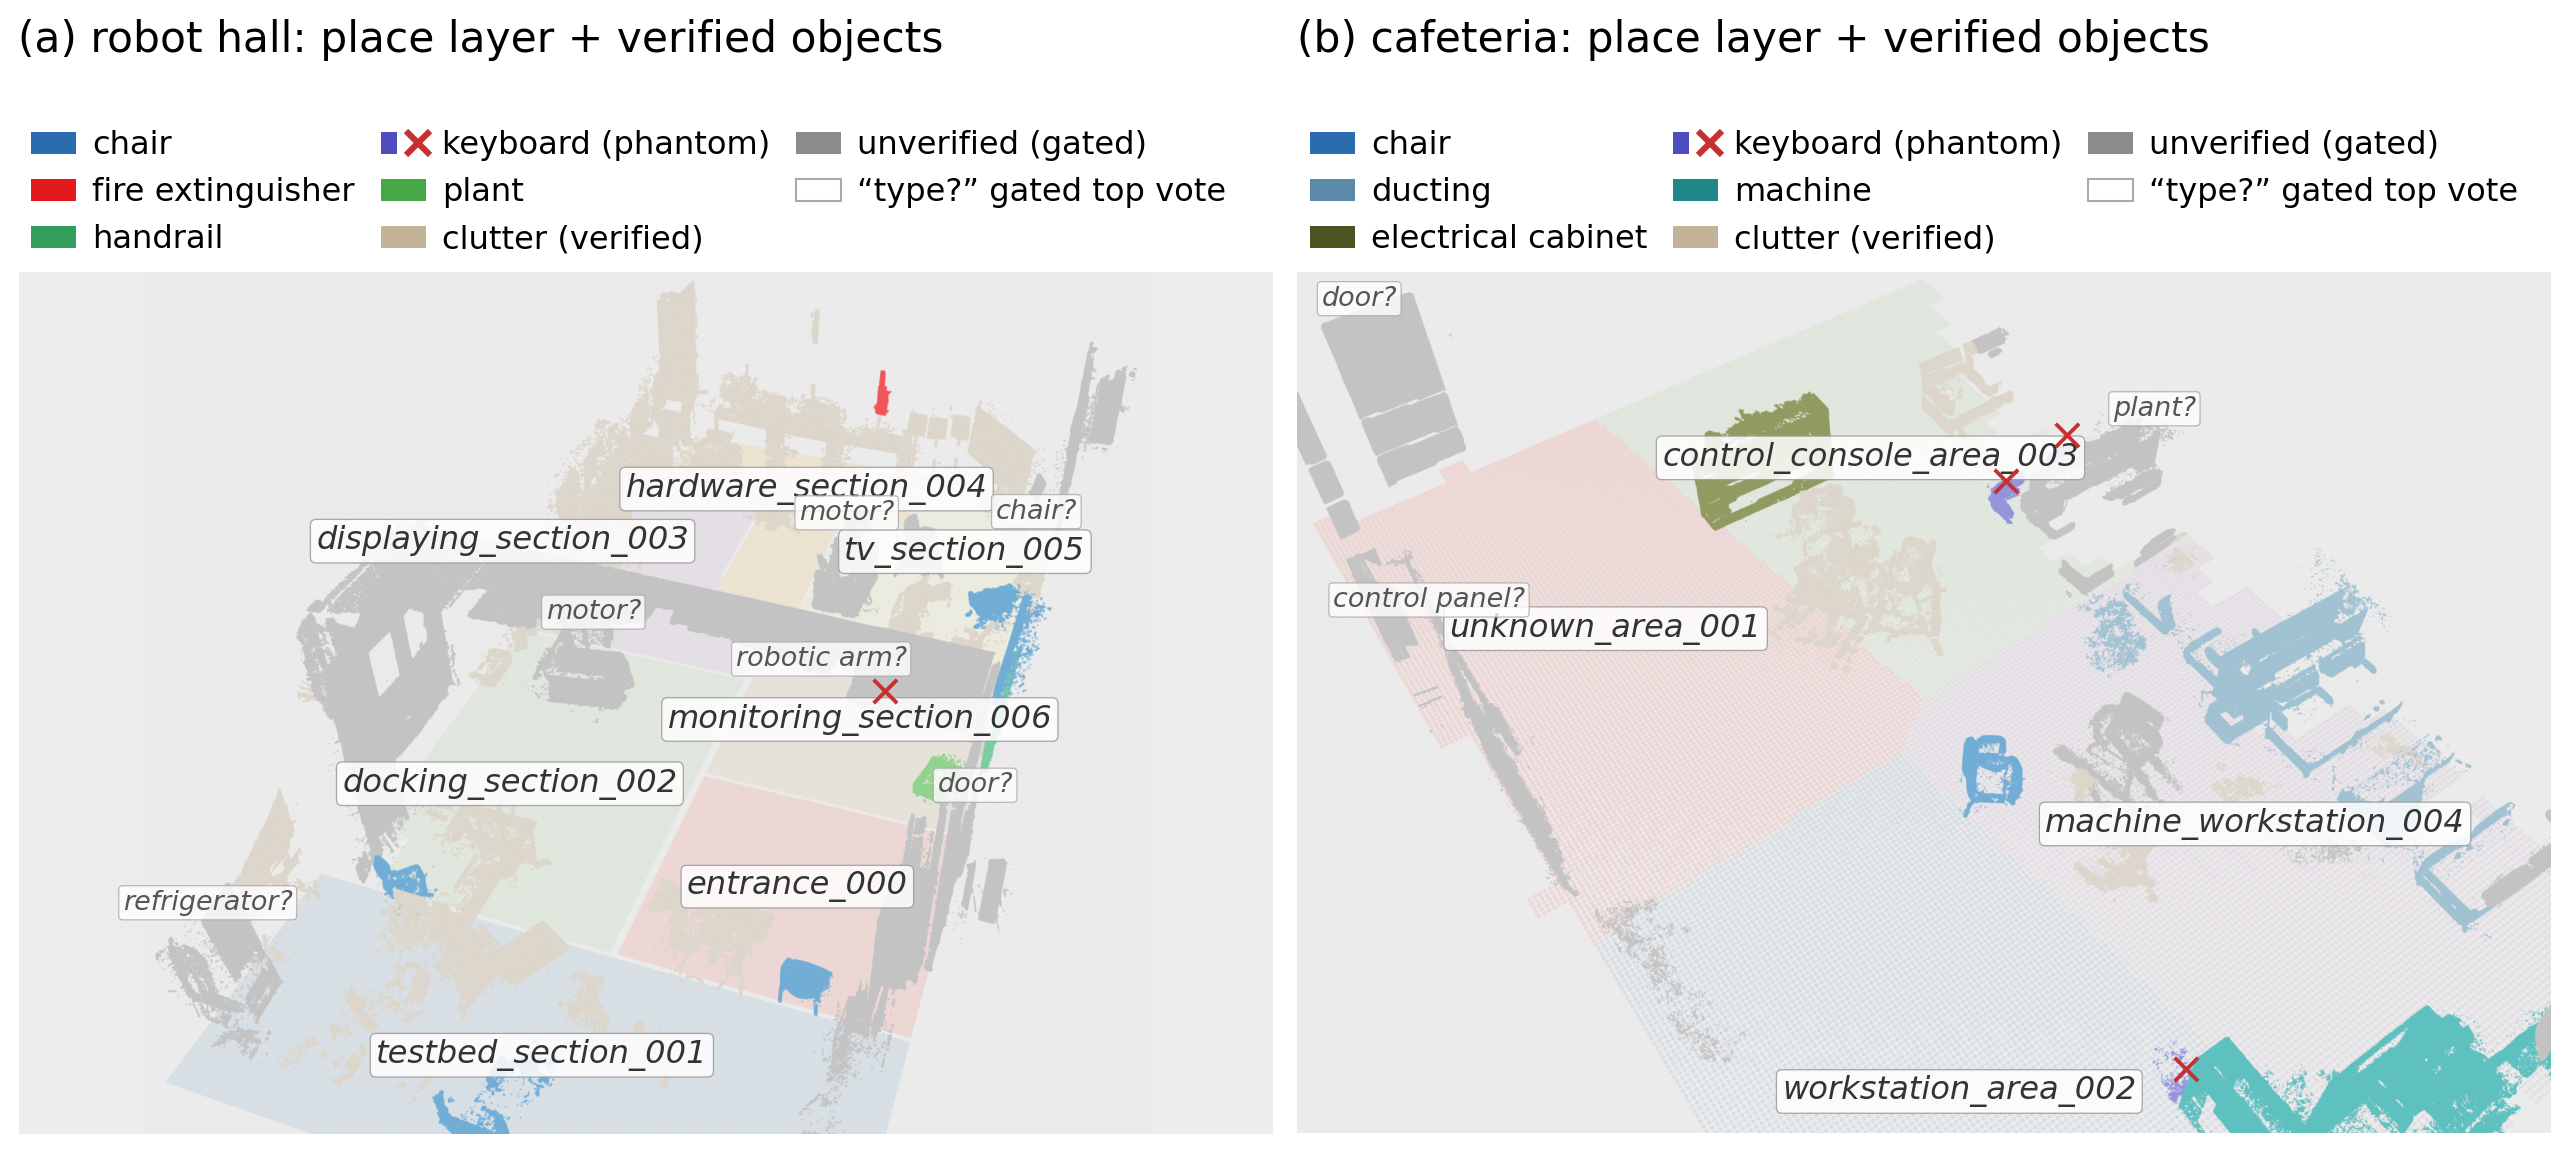
\includegraphics[width=\linewidth]{figures/ele_fig19_semantic_map.png}
\caption{The generated semantic map, visualized at the verification stage
(before owner feedback), so the confidence gate and the errors that pass it
are both visible. (a)~Robot hall: SLIC place-layer regions (pastel floor) with
the room-scoped object clusters rendered as their segmented points, colored by
verified class; gray clusters are \texttt{unverified} and demoted at query
time. (b)~The cafeteria stress scene under the same representation; red
crosses mark verified-keyboard clusters that are owner-refuted phantoms.}
\label{fig:semmap}
\end{figure}

\section{Digital Twin: Conversion, Performance, and Fidelity}
\label{sec:exp-twin}

All twin experiments ran on the desktop workstation of
Section~\ref{subsec:platforms} (Isaac Sim~5.1, ROS~2 Jazzy).

\paragraph{Conversion time and resources.}
Table~\ref{tab:convtime} reports single-run wall-clock times for each pipeline
stage on the 68.5~M-point scan. The complete conversion from raw E57 to a
simulation-ready USD stage takes 78.5~s; the dominant cost is writing the
3.7~M-point visual layer, and a reduced-density variant (485~K points)
completes in 36.5~s. The conversion runs entirely on the CPU, peaking at 8.1~GB
of resident memory with an average utilization of 2.4 cores; the simulator
process occupies 3.1~GB of GPU memory with the full scene and robot
articulation loaded in headless physics-only mode. Authoring a comparable
environment by hand is a multi-day effort, and, unlike manual modeling, the
pipeline can be rerun after every facility change. Every stage is linear in
the number of input points, so conversion time scales roughly linearly with
scan size; the main memory constraint is holding the merged cloud in RAM,
which for facility-scale scans beyond roughly $10^8$ points would call for
chunked streaming of the E57 input.

\begin{table}[htbp]
\centering
\caption{Scan-to-simulation conversion time (68.5~M-point E57). Source:
RAAICON~2026~\cite{raaicon2026}.}
\label{tab:convtime}
\begin{tabular}{l r}
\toprule
\textbf{Stage} & \textbf{Time (s)} \\
\midrule
Floor RANSAC, occupancy grid, ROS map export & 14.8 \\
Dense visual cloud extraction (voxel 0.015~m) & 16.8 \\
Visual layer USD export (3.7~M points) & 46.8 \\
Collision-layer synthesis (1{,}430 boxes) & 0.1 \\
\midrule
\textbf{Total} & \textbf{78.5} \\
\bottomrule
\end{tabular}
\end{table}

\paragraph{Scene complexity and simulation performance.}
The generated stage contains 1{,}430 collision boxes ($\approx$17~K
triangles) and 3{,}725{,}047 rendered points (166~MB USD). With the AMMR
articulation loaded (physics at 120~Hz), headless physics-only simulation
advances at 675 steps/s, a real-time factor of 5.6; with rendering enabled the
simulator sustains 51 rendered frames per second (real-time factor 0.84), and
in the interactive GUI session used for the on-site experiments the viewport
sustained 104 frames per second with the full point layer in view. Before
coupling to the real robot, the swerve base was validated in simulation:
straight-line (1.13~m forward run), lateral (1.45~m strafe), and in-place
rotation ($65^{\circ}$) maneuvers each produced odometry matching the
commanded motion direction, and the flip hysteresis of
Equation~\ref{eq:swerve} eliminated the wheel-speed oscillation otherwise
observed at steering-wrap boundaries.

\paragraph{Live twin verification and simulator-issued goals.}
The bridge contract was verified end to end with the physical AMMR in the
scanned facility (Figure~\ref{fig:pairroom}): the 30~Hz state stream is
received across the Wi-Fi link, the anchor calibration of
Equation~\ref{eq:anchor} converges from a single pose sample, and goals picked
in the simulator drive the real robot through Nav2. During the on-site session
the twin mirrored teleoperated motion continuously across a 3.4~m sweep of the
room. Across two sessions on consecutive days, all four navigation goals
issued by dragging the target marker in the simulator viewport drove the robot
to the corresponding physical locations (Table~\ref{tab:goaltrials},
Figure~\ref{fig:pairgoal}); the twin-frame arrival error of 0.19--0.23~m
(mean 0.21~m) is consistent with the Nav2 goal tolerance, at commanded speeds
up to 0.52~m/s.

\begin{table}[htbp]
\centering
\caption{Simulator-issued navigation-goal trials on the physical AMMR.
Source: RAAICON~2026~\cite{raaicon2026}.}
\label{tab:goaltrials}
\begin{tabular}{c c c l}
\toprule
\textbf{Trial} & \textbf{Session} & \textbf{Error (m)} & \textbf{Note} \\
\midrule
1 & day 1 & 0.19 & 14.4~s run \\
2 & day 1 & 0.21 & \\
3 & day 2 & 0.19 & \\
4 & day 2 & 0.23 & 3.0~m straight, up to 0.52~m/s \\
\midrule
\multicolumn{2}{l}{\textbf{Mean (4/4 reached)}} & \textbf{0.21} & \\
\bottomrule
\end{tabular}
\end{table}

\begin{figure}[!htb]
\centering
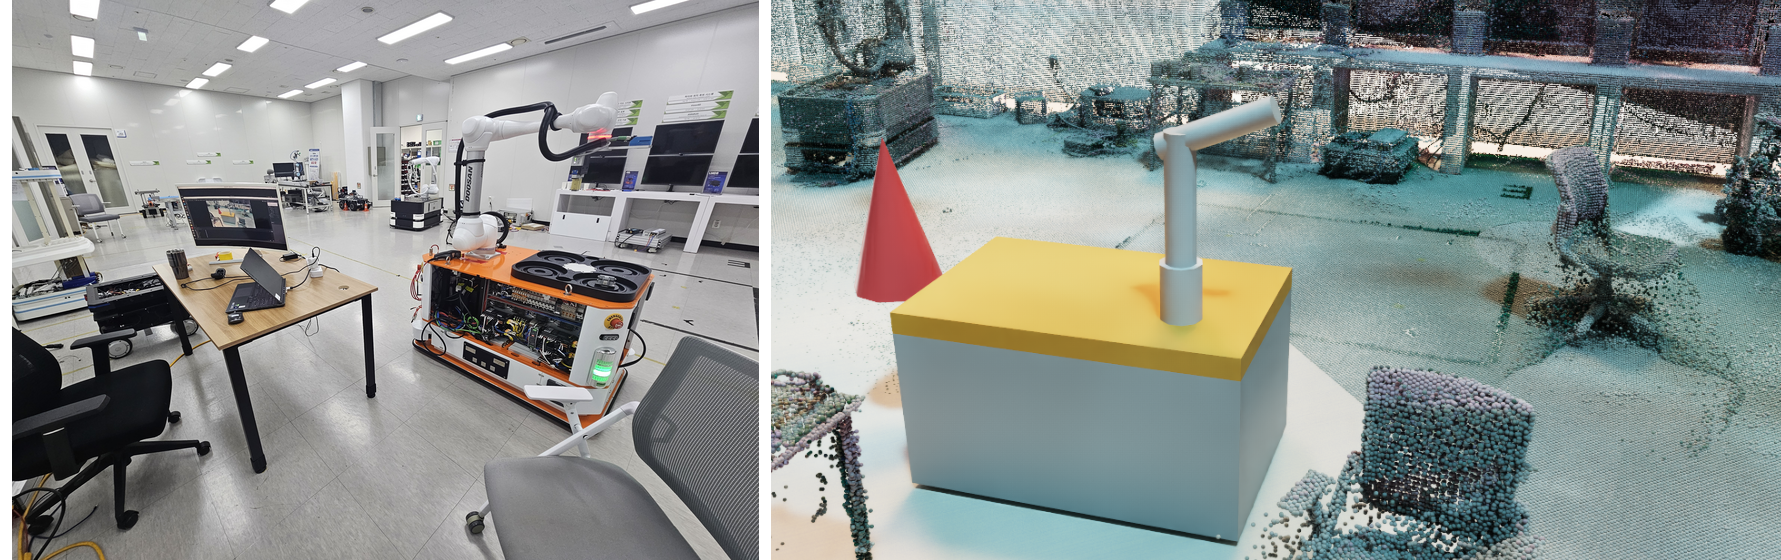
\includegraphics[width=0.95\linewidth]{figures/raa_fig_pair_room.png}
\caption{Test facility (left) and its generated twin during the live session
(right). The yellow body with the white column is the AMMR proxy model; the
red cone is the draggable navigation-goal marker.}
\label{fig:pairroom}
\end{figure}

\begin{figure}[!htb]
\centering
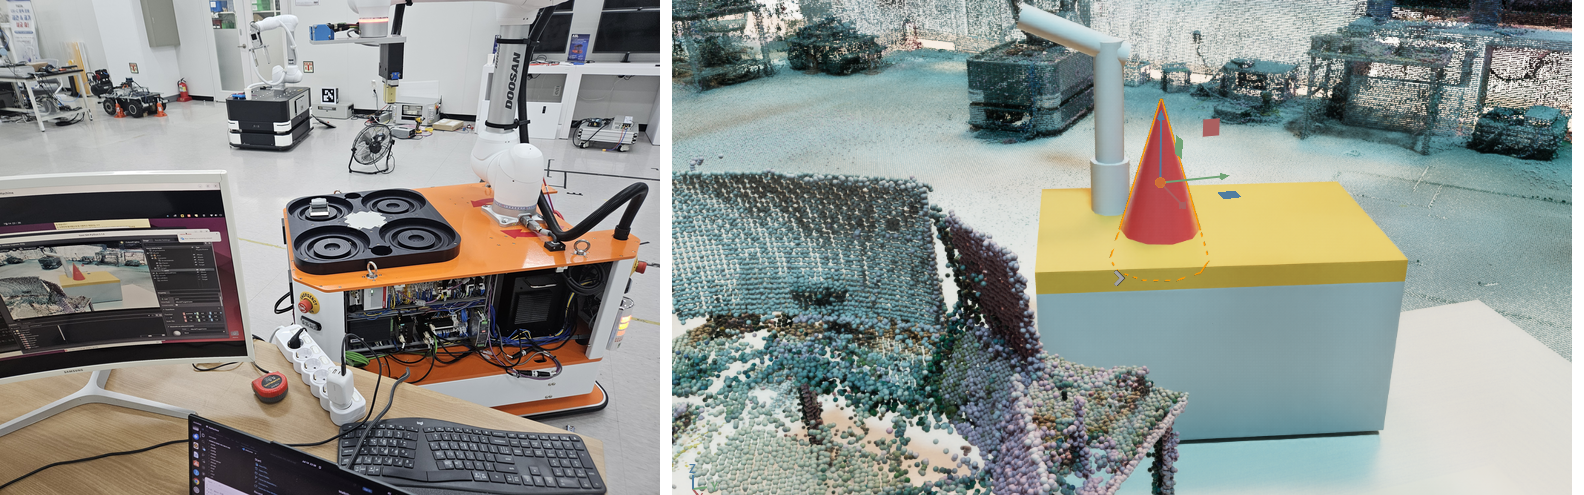
\includegraphics[width=0.95\linewidth]{figures/raa_fig_pair_goal.png}
\caption{Simulator-issued navigation goal. Left: the physical robot at the
reached location; right: the twin after arrival, parked on the goal marker.}
\label{fig:pairgoal}
\end{figure}

\paragraph{Geometric fidelity.}
Metric accuracy is evaluated at two levels. Three room features were
tape-measured and compared against the same dimensions extracted from the
twin's point layer (Table~\ref{tab:geo}): all errors are within 2\% (mean
absolute error 6.4~cm, or 1.3\%), so the scan-to-simulation conversion itself
preserves metric scale to centimeter level. End to end, tape-measured
distances between marked floor checkpoints were compared against the
corresponding distances reported by the twin with the robot parked on each
checkpoint, which captures the full error budget---TLS registration, occupancy
quantization, AMCL localization, and anchor calibration---without requiring a
global frame alignment. Over three checkpoint pairs (0.86, 3.14, and 1.30~m
tape distance) the twin distances deviated by a mean absolute error of 5.5~cm
(RMSE 7.4~cm, maximum 12.5~cm, signed bias $+2.8$~cm; Figure~\ref{fig:eval}).
The largest deviation occurred on the segment executed with large in-place
rotations and matches the AMCL repeatability observed when revisiting the same
floor marker (17~cm), indicating that end-to-end twin accuracy is dominated by
the onboard localization rather than by the reconstructed scene.

\begin{table}[htbp]
\centering
\caption{Scene-feature dimensions: tape measure vs.\ twin point layer.}
\label{tab:geo}
\begin{tabular}{l r r r}
\toprule
\textbf{Feature} & \textbf{Real (m)} & \textbf{Twin (m)} & \textbf{Error} \\
\midrule
Window-side wall length & 8.000 & 7.918 & $-1.0$\% \\
Double-door width & 1.700 & 1.680 & $-1.2$\% \\
Workbench row length & 5.010 & 5.100 & $+1.8$\% \\
\bottomrule
\end{tabular}
\end{table}

\begin{figure}[!htb]
\centering
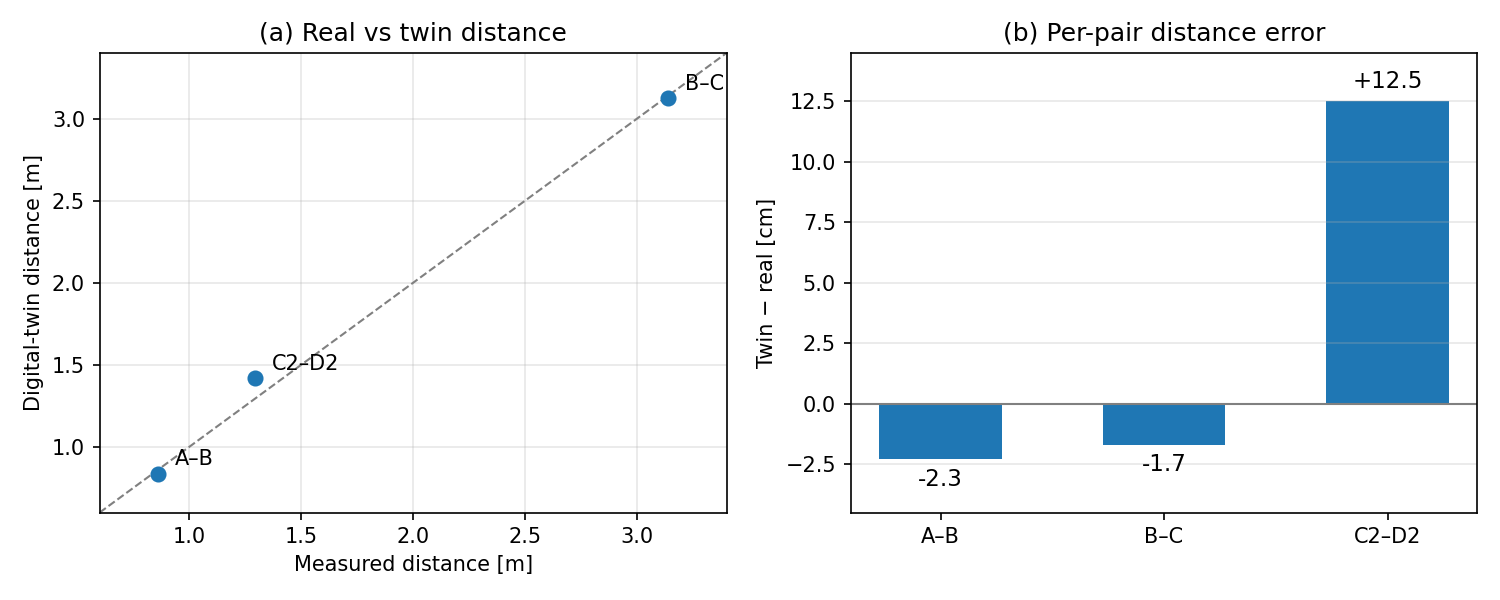
\includegraphics[width=0.95\linewidth]{figures/raa_fig_eval.png}
\caption{Checkpoint-pair distances, tape measure vs.\ twin: scatter against
the identity line (left) and signed per-pair error (right).}
\label{fig:eval}
\end{figure}

\section{Semantic Mission Execution in Simulation and on the Physical Robot}
\label{sec:exp-missions}

\paragraph{Simulation.}
In the Gazebo twin of the test room, over three repetitions of a
three-mission battery (approach the TV, go to the seating area, return home),
task success is 9/9, with mean leg path lengths 4.6/5.4/1.8~m and completion
times 16.5/24.9/15.0~s; semantic resolution latency (command to accepted or
refused goal) is under one second, and a gate refusal stops the robot safely
with zero motion. The reactive layer supplies the safety-stop behavior: a
low-battery event during navigation preempts the active Nav2 goal and returns
the platform to a holding position at home. The phantom experiment
(Table~\ref{tab:semnav}) sends the robot to three owner-refuted phantoms under
two knowledge states. Against the pre-feedback graph, all three phantoms carry
\emph{verified} labels, so the confidence gate passes them---and the waste
takes three distinct forms: a pointless drive to a fluorescent lamp; a
\emph{false arrival} at a 7.4~m ``staircase'' whose approach ring encloses the
robot's own position; and 22~s of futile replanning toward a wall-pillar
``book'' whose approach pose the platform's footprint cannot reach. Against the
graph after structure filtering and owner feedback, the same commands are
refused in about one second with zero motion (Figure~\ref{fig:semnav}).
Verification gating alone cannot stop verified phantoms; it is the combination
of gating, structure-noise removal, and owner feedback that reduces the robot's
exposure to phantom semantic claims.

\begin{table}[htbp]
\caption{Phantom-goal mission waste in simulation (AMMR proxy). The same three
commands are resolved against the knowledge graph before and after structure
filtering + owner feedback (both with the verification gate active).}
\label{tab:semnav}
\centering
\begin{tabular}{l l c c c}
\toprule
\textbf{KG state} & \textbf{Phantom target (truth)} & \textbf{Outcome} & \textbf{Wasted path} & \textbf{Wasted time} \\
\midrule
pre-feedback & keyboard (fluorescent lamp) & driven & 1.7~m & 16.8~s \\
pre-feedback & staircase (bare wall) & false arrival & 0.6~m & 5.7~s \\
pre-feedback & book (wall pillar) & unreachable, aborted & 0~m & 22.2~s \\
\midrule
filtered + owner feedback & all three & refused & 0~m & $\sim$1~s \\
\bottomrule
\end{tabular}
\end{table}

\begin{figure}[!htb]
\centering
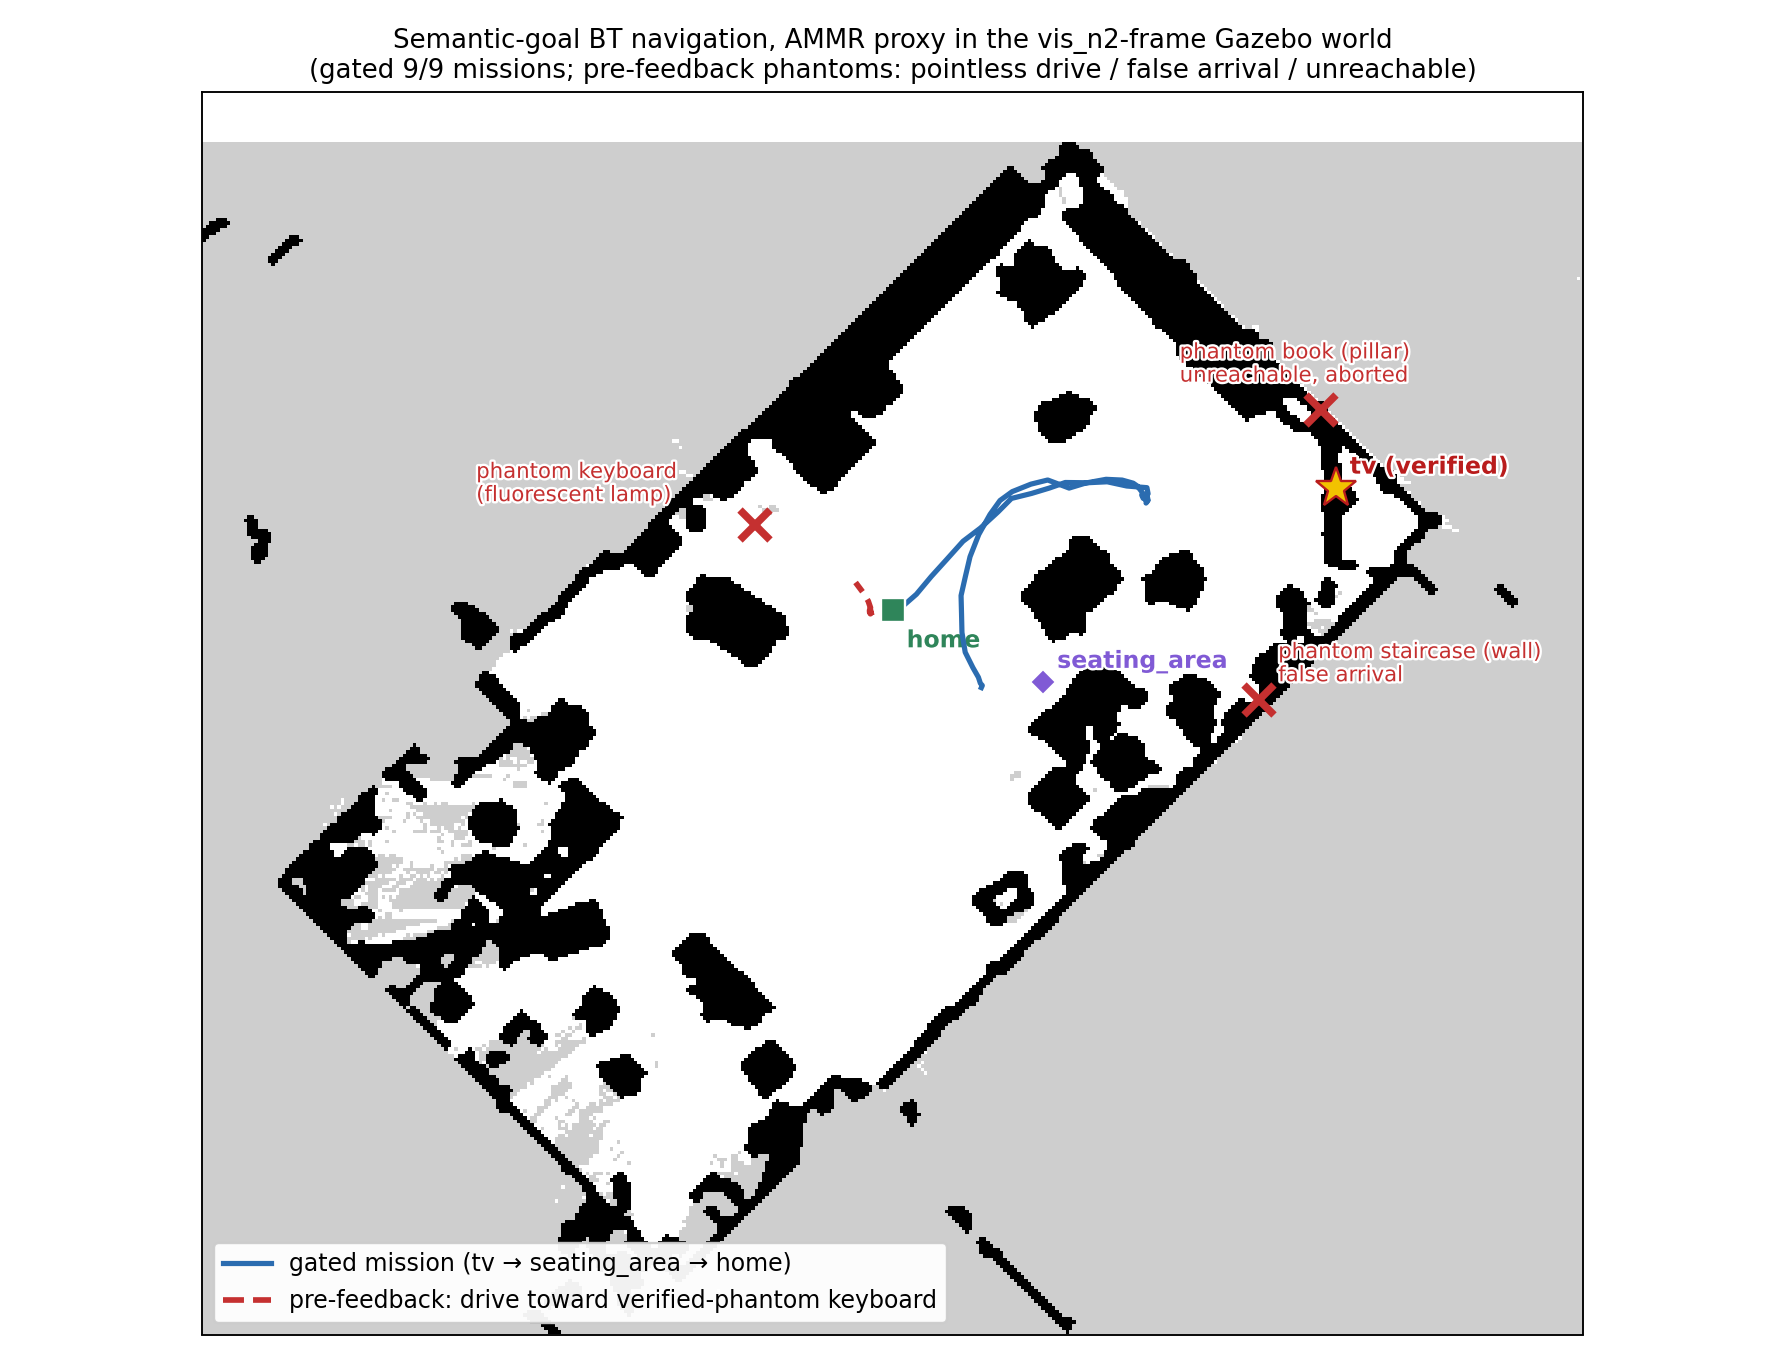
\includegraphics[width=0.8\linewidth]{figures/ele_fig15_semantic_nav_run.png}
\caption{Semantic-goal navigation of the AMMR proxy in the Gazebo twin of the
test room. Blue: a gated three-mission run (TV $\rightarrow$ seating area
$\rightarrow$ home). Red dashed: against the pre-feedback graph the robot
drives toward a verified-phantom keyboard; crosses mark the three phantom goals
with their failure modes. All three are refused once structure filtering and
owner feedback are applied.}
\label{fig:semnav}
\end{figure}

\paragraph{Physical robot.}
The mission stack was run unchanged against the physical AMMR in the test
room (robot-hall configuration) through the bridge of
Section~\ref{sec:real-robot}, with the console, the Isaac Sim twin, and the
robot all served from the same knowledge graph. Three semantic drives
completed---two \texttt{goto\_object} approaches to the wall TV and one
\texttt{goto\_place} drive into the monitor workstation region, each
3.6--4.0~m from the start---in 14--22~s with arrival errors of 0.22--0.34~m
(mean 0.30~m) between the robot's localized pose and the resolved goal; a
place command issued while the robot already stood inside the region completed
without motion (0.11~m from the region goal). The gate behaved as in
simulation: \texttt{goto\_object keyboard}, the owner-refuted phantom of
Table~\ref{tab:semnav}, was refused by the mediator in under one second with
zero robot motion, twice (Table~\ref{tab:realrobot},
Figure~\ref{fig:realrobot}). Missions were issued one at a time from a standing
start. The exercise is a bounded validation---one room, one platform, three
completed drives---but it confirms that the graph that survives verification,
gating, and owner feedback is directly consumable by a real robot, and that the
twin, console, and robot stay consistent because they read one store.

\begin{table}[htbp]
\caption{Real-robot semantic missions on the AMMR (test room, 15 September
2026). Goals are resolved by the mediator in the scan frame; distance is
straight-line start-to-goal; arrival error is the localized-pose-to-goal
distance at mission completion. Source: \emph{Electronics}~\cite{kim2026electronics}.}
\label{tab:realrobot}
\centering
\footnotesize
\begin{tabularx}{\textwidth}{X l c c c X}
\toprule
\textbf{Command} & \textbf{Resolved goal (m)} & \textbf{Dist.} & \textbf{Time} & \textbf{Err.} & \textbf{Outcome} \\
\midrule
\texttt{goto\_object tv} & tv\_006 (3.09, 1.91) & 4.0~m & 14~s & 0.34~m & completed \\
\texttt{goto\_object tv} (Fig.~\ref{fig:realrobot}a) & tv\_006 (3.09, 1.91) & 3.6~m & 20.8~s & 0.33~m & completed \\
\texttt{goto\_place electrical\_ maintenance\_area} (Fig.~\ref{fig:realrobot}b) & region ($-$0.69, 3.81) & 3.9~m & 22.1~s & 0.22~m & completed \\
\texttt{goto\_place display\_ briefing\_area} & region (3.31, 1.76) & 0.1~m & $<$1~s & 0.11~m & completed (already inside) \\
\texttt{goto\_object keyboard} ($\times$2, phantom) & --- & --- & $<$1~s & --- & refused by gate, no motion \\
\bottomrule
\end{tabularx}
\end{table}

\begin{figure}[!htb]
\centering
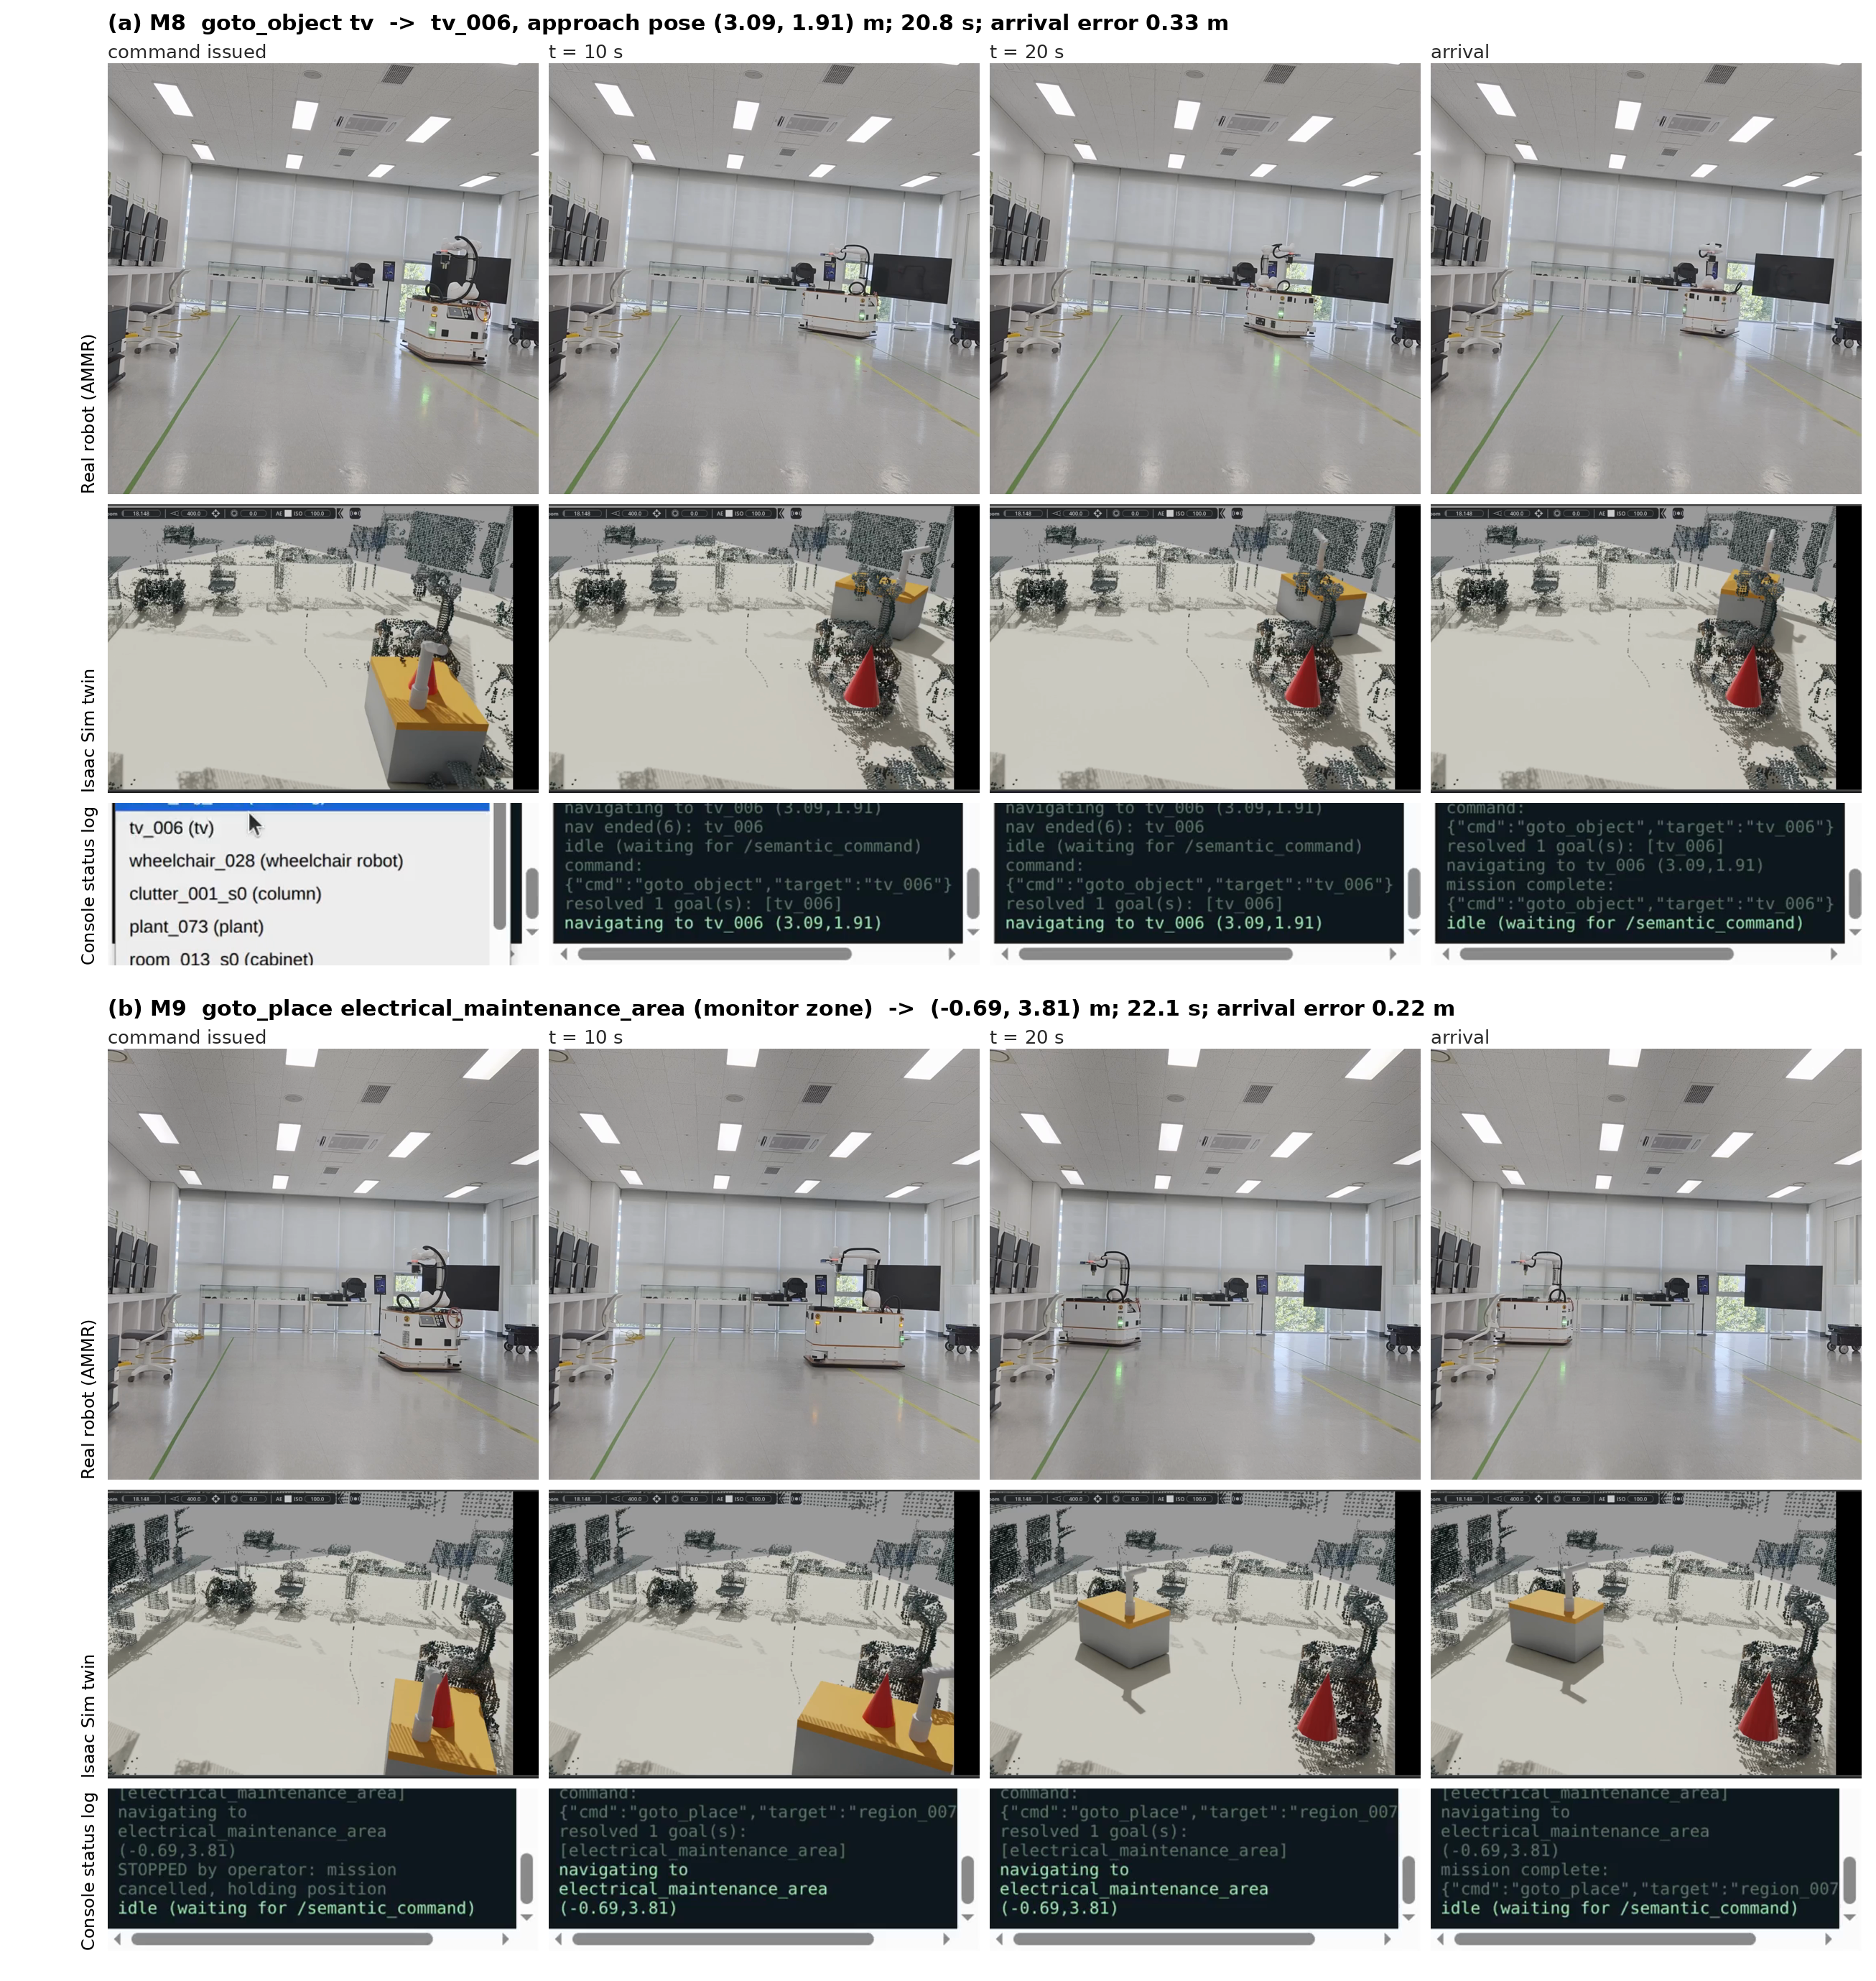
\includegraphics[width=\linewidth]{figures/ele_fig20_real_robot_missions.png}
\caption{Real-robot semantic missions (Table~\ref{tab:realrobot}). Rows: the
physical AMMR, the Isaac Sim twin derived from the same knowledge graph (the
red cone marks the twin's goal handle), and the management console's status
log; columns: command issued, 10~s, 20~s, and arrival. (a)~\texttt{goto\_object
tv}: the mediator resolves the verified node \texttt{tv\_006} to an approach
pose and the robot arrives 0.33~m from it in 20.8~s. (b)~\texttt{goto\_place
electrical\_maintenance\_area}: the region containing the monitor workstation,
reached in 22.1~s with 0.22~m error.}
\label{fig:realrobot}
\end{figure}

\section{Overhead Layer: Ceiling-Mounted Structure}
\label{sec:exp-overhead}

The overhead recognition pass of Section~\ref{sec:overhead} was run with its
parameters frozen on the two industrial epochs (T2, T3) and on the cafeteria
scene. Table~\ref{tab:overhead} summarizes the outcome of each stage and
Figure~\ref{fig:overhead} shows the T3 result over the floor-level graph.

\begin{table}[htbp]
\centering
\caption{Overhead recognition pass on three scenes (parameters frozen; the
verifier and protocol of Section~\ref{sec:exp-verify}). ``Cut'' = clusters
whose bottom lies at the band cut and are dropped as truncated continuations
of floor-level content; in-room = inside the room mask with the 0.5~m wall
tolerance.}
\label{tab:overhead}
\footnotesize\setstretch{1.15}
\begin{tabularx}{\textwidth}{X c c c}
\toprule
 & \textbf{Robot hall (T2)} & \textbf{Re-scan (T3)} & \textbf{Cafeteria} \\
\midrule
Reference cloud (points) & 989~K & 995~K & 546~K \\
Overhead-band points ($>$1.8~m) & 545~K & 512~K & 241~K \\
Ceiling levels found (m above floor) & 3.00 / 3.20 / 3.52 & 3.00 / 3.17 / 3.49 & 3.00 \\
Wall planes & 7 & 6 & 7 \\
Candidate points after ceiling/wall removal & 28.0~K & 39.6~K & 1.4~K \\
Floor-connected candidate points removed & 12.4~K & 31.4~K & 1.2~K \\
Clusters (after cut rule) & 18 & 12 & 0 \\
In-room objects & 5 & 6 & 0 \\
Verified unanimous / escalated / unverified & 1 / 4 / 0 & 1 / 3 / 2 & --- \\
VLM calls / cost & 57 / \$0.55 & 70 / \$0.67 & --- \\
\bottomrule
\end{tabularx}
\end{table}

\begin{figure}[!htb]
\centering
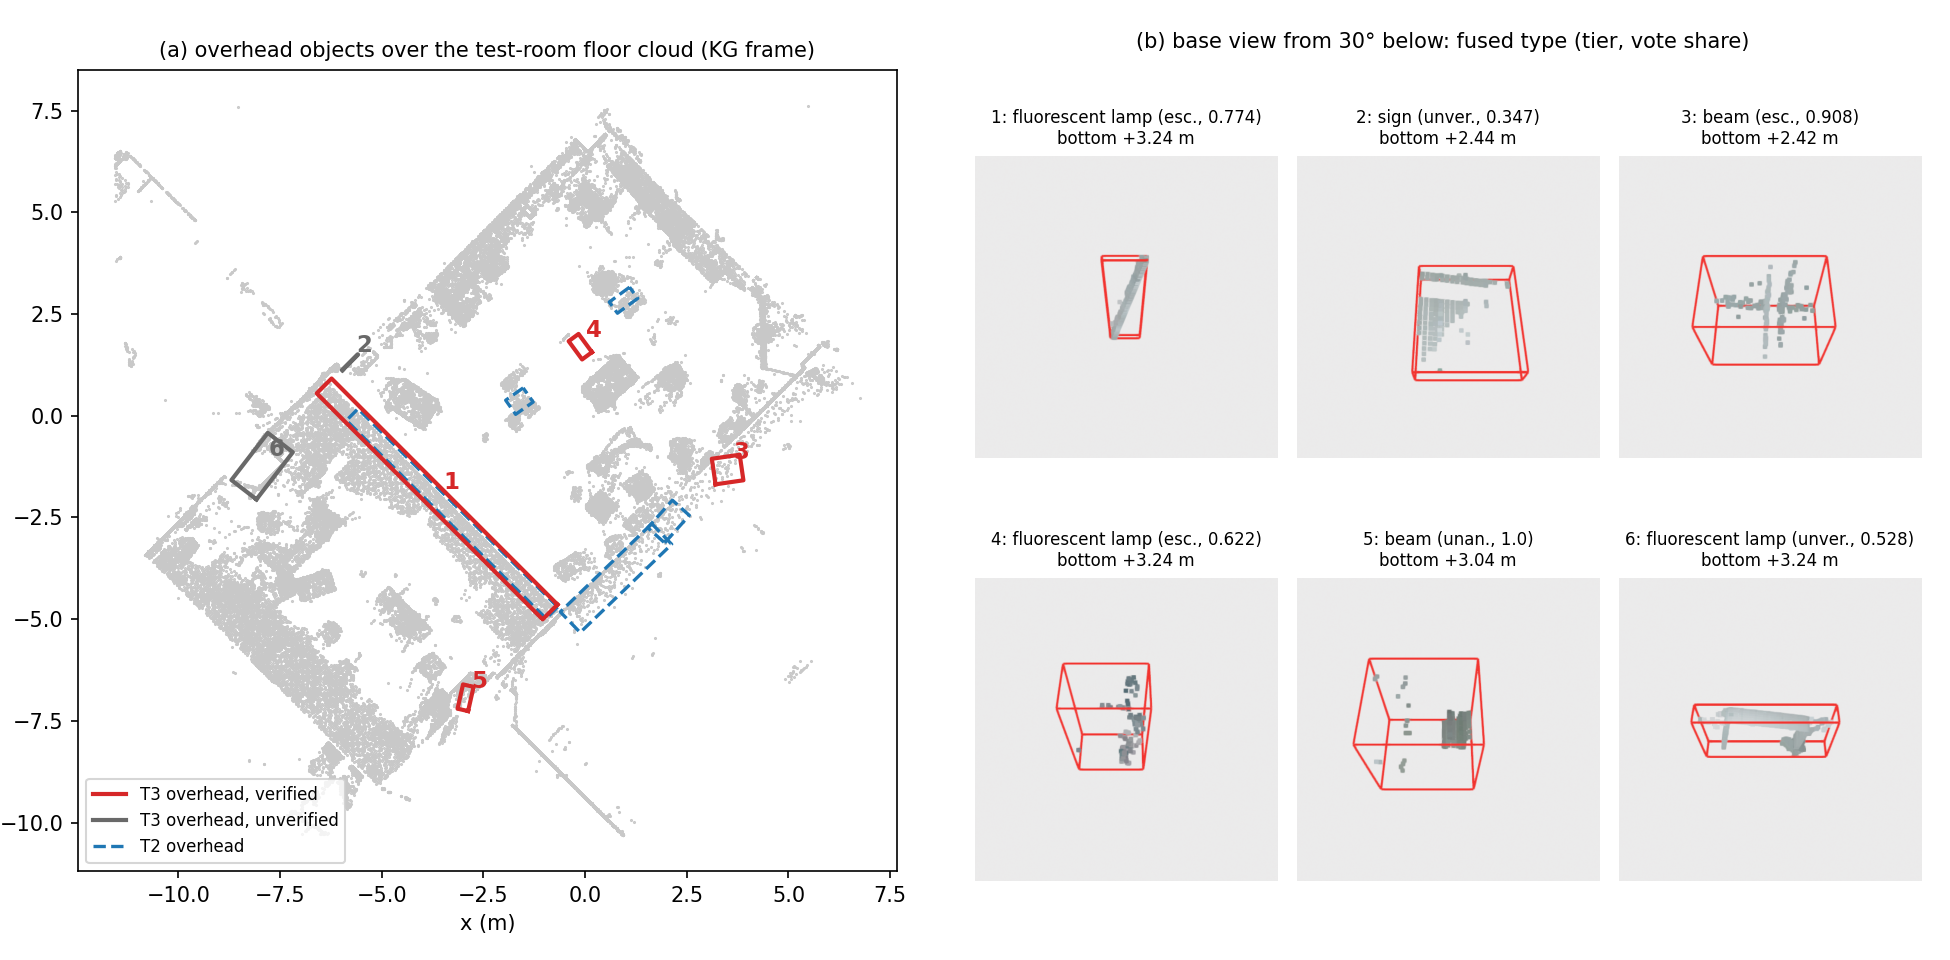
\includegraphics[width=\linewidth]{figures/fig6_overhead.png}
\caption{Overhead layer on the T3 epoch. (a)~The six in-room overhead objects
(red: verified tiers, gray: unverified) over the floor-level cloud, with the
five T2 overhead objects dashed in blue; (b)~each object's base render from
$30^\circ$ below with its fused type, tier, and vote share.}
\label{fig:overhead}
\end{figure}

\paragraph{What the pass finds.}
On T3 the pass isolates six in-room overhead objects: a 7.9~m lighting rail
0.25~m below the top ceiling level (verified as a fluorescent lamp by
escalation), three small fixtures at the same height (one verified
unanimously as a \emph{beam}, one as a fluorescent lamp by escalation, and
one left unverified with \emph{fluorescent lamp} at share 0.53), a hanging
thin plate 2.4~m above the floor (unverified; \emph{sign} at share 0.35),
and a sparse cross-shaped pipe junction (verified as \emph{beam} by
escalation). Every in-room object is attached to a ceiling level
(\emph{ceiling-hung}); the wall-mounted and suspended categories occur only
outside the room. Four of the six are verified (one unanimously, three by
escalation) and two remain unverified, at a cost of under \$1 for the scene.
On T2, the same room scanned from the
robot deck nine days earlier, the pass finds five in-room objects, all
verified (one unanimously, four by escalation). On the cafeteria the pass
finds \emph{nothing}: its single flat ceiling at 3.0~m carries recessed
lights that lie inside the ceiling band, and the 1.4~K candidate points that
survive ceiling and wall removal all belong to floor-connected clusters. A
null result on a scene that has no hanging structure is the intended
behavior of the pass, and it is reported as such.

\paragraph{Ground truth.}
\textcolor{red}{[Owner ground truth for the eleven T3 candidates (union of
the two extraction rules below) is being collected on the sheet
\texttt{overhead\_gt\_sheet.csv}; the precision figures of this paragraph
will be filled in from it.]} A render audit by the author, under the same
protocol as the floor-level audit, grades the lighting rail, the three
fixtures at the top level, the hanging plate, and the pipe junction as
plausible overhead objects; as for the floor pass, render-only annotation
cannot resolve fixture \emph{types} (a lamp housing and a cable tray look
alike from below at 3~cm spacing), so the type precision of the tiers is
reported only against the owner's inventory.

\paragraph{Extraction rule and its alternative.}
The frozen rule decides that a candidate is overhead by connectivity: a
cluster that reaches down into the driving band through the structure-free
lower cloud (at $\varepsilon=0.15$~m) is the upper part of a floor object. An
alternative rule, tested first, excludes candidate points that fall inside
the footprint of a floor-pass object beneath them; on T3 it returned nine
in-room candidates instead of six, because three fixtures that hang within
0.15~m of wall-mounted equipment (a projector-like bracket near the display
wall, a hanging rack, and a boxed unit) are absorbed by the connectivity
test, but on T2 it failed outright: the footprints of that epoch's merged
mega-clusters (Section~\ref{subsec:exp-params}) covered most of the room and
suppressed every fixture. Connectivity is therefore retained as the frozen
rule, and the owner sheet lists the union of both candidate sets so that
the recall cost of the connectivity rule can be scored.

\paragraph{Identity across epochs.}
Overhead objects are the most static content of a room, which makes them a
clean test of the identity policy of Section~\ref{sec:matching}. Upserting
the T2 set and then the T3 set into an overhead graph gives, for the T3
epoch, 0 matched, 1 moved, 5 inserted, and 4 absent. The reason is not
matching but coverage: the two scans see different parts of the ceiling. The
robot-deck exploration scan (T2) resolves the lighting rail and two fixtures
near the room center, whereas the six-setup re-scan (T3) resolves the rail
plus fixtures at the room's ends; only the rail is common to both, and its
centroid shifts by 0.52~m between the epochs because T2 captured 6.9~m of it
and T3 7.9~m---just outside the 0.5~m spatial gate, so the rail is
re-inserted under a new identity (the fragmentation error class of
Section~\ref{sec:exp-update}), and one same-type pair 1.9~m apart is
recorded as a false move. Two conclusions follow. First, ceiling coverage
depends on station placement at least as much as floor coverage does, so
the overhead layer inherits the coverage sensitivity of Part~A. Second,
elongated fixtures need an extent-overlap matching feature rather than a
centroid gate; this is the same feature the floor-level occlusion scenario
of Section~\ref{sec:exp-update} motivated, and it is left to future work.

\paragraph{Consumption.}
Verified overhead objects enter the knowledge graph with
\texttt{heightLevel = high}, their clearance below (2.4--3.2~m in the test
room), and their attachment, and the console and the Isaac Sim twin derive
them from the same store as every other node; a pointing or installation
task resolves against a verified overhead node exactly as a navigation task
resolves against a floor node, with the same gate refusing unverified ones.
No lifting platform executed such a task in this dissertation
(Chapter~\ref{ch:conclusion}).

\section{Summary against the Research Objectives}
\label{sec:exp-summary}

Table~\ref{tab:objsummary} maps the principal results of this chapter back to
the five research objectives of Section~\ref{sec:objectives} and states the
scope of each result.

\begin{table}[htbp]
\centering
\caption{Principal results against the research objectives, with scope.}
\label{tab:objsummary}
\small
\begin{tabularx}{\textwidth}{l X X}
\toprule
\textbf{Obj.} & \textbf{Principal result} & \textbf{Scope} \\
\midrule
O1 & Visibility rule: LOS $77\%\to84$--$85\%$ (paired ablation, $+1$--2 scans); on hardware $77.6\to92.1\%$; all visibility runs register at 4--5~mm bundle error, 84--88\% overlap & Room-scale indoor, 2D visibility, one scanner, one test room \\
O2 & Byte-identical backbone across hosts; recall 0.952 vs.\ owner inventory at the operating point; learned closed-set/projection baselines fail on industrial content & Proxy metrics for baseline screening; one industrial scene \\
O3 & Escalation $77.8\to88.9\%$ / $78.1\to84.4\%$; unanimity 94--100\% precision; gated query 83.3\% with 3/4 traps blocked; zero identity switches over three epochs; re-verification at 3.1\% of rebuild; automated recall $28\to85\%$ & One building; tier precision is scene-scoped (cafeteria 35--60\%); replay on development scene \\
O4 & Scan-to-sim in 78.5~s; RTF 5.6 physics-only, 104~FPS viewport; dimensions within 2\%; end-to-end positioning 5.5~cm MAE; overhead layer: 6 in-room ceiling objects on T3 (5 verified), null result on the flat-ceiling cafeteria & One room; overhead band validated at the representation level, not with a lift \\
O5 & Simulator-issued goals 4/4 (0.21~m); console-issued semantic missions 3 completed (0.30~m mean error), 2 phantom refusals with zero motion; twin, console, robot consistent from one store & One platform (AMMR), missions from a standing start \\
\bottomrule
\end{tabularx}
\end{table}
